\documentclass[aspectratio=169,10pt]{beamer}

% Author at a true presentation canvas so absolute overlays and raster donors
% share the same 16:9 geometry instead of Beamer's small default physical page.
\setlength{\paperwidth}{13.333in}
\setlength{\paperheight}{7.5in}
\geometry{paperwidth=13.333in,paperheight=7.5in}

\usepackage[T1]{fontenc}
\usepackage{tgpagella}
\usepackage[scale=0.94]{tgheros}
\usepackage{amsmath,amssymb,bm}
\usepackage{graphicx}
\usepackage{tikz}
\usetikzlibrary{arrows.meta,calc,positioning,shapes.geometric}

\setbeamertemplate{navigation symbols}{}
\setbeamertemplate{footline}{}
\setbeamertemplate{headline}{}
\setbeamersize{text margin left=0.48in,text margin right=0.48in}

\definecolor{ink}{HTML}{102446}
\definecolor{teal}{HTML}{0D8383}
\definecolor{blue}{HTML}{2D67B1}
\definecolor{purple}{HTML}{7656C8}
\definecolor{orange}{HTML}{EF8C3A}
\definecolor{green}{HTML}{2F9D76}
\definecolor{red}{HTML}{D95F59}
\definecolor{muted}{HTML}{687384}
\definecolor{warm}{HTML}{FBFAF6}
\definecolor{paleteal}{HTML}{EAF6F4}
\definecolor{paleblue}{HTML}{EAF1FA}
\definecolor{palepurple}{HTML}{F1EDFA}
\definecolor{paleorange}{HTML}{FFF4E8}
\definecolor{palered}{HTML}{FCEDEC}

\setbeamercolor{background canvas}{bg=warm}
\setbeamercolor{normal text}{fg=ink,bg=warm}
\setbeamercolor{frametitle}{fg=ink,bg=warm}
\setbeamerfont{frametitle}{family=\rmfamily,series=\bfseries,size=\fontsize{24}{27}}
\setbeamerfont{normal text}{family=\sffamily,size=\fontsize{11}{14}}

\setbeamertemplate{frametitle}{%
  \vspace{0.12in}%
  \insertframetitle\par
  \vspace{0.04in}%
  {\color{ink!82}\rule{\textwidth}{0.9pt}}%
}

\graphicspath{{../canvas_assets/}{../canvas_assets/extra/}{../canvas_assets/newg/}{../ml_workshop_15_20min/assets/}{assets/}}

\newcommand{\fullimage}[1]{%
  \begin{tikzpicture}[remember picture,overlay]
    \node[anchor=center,inner sep=0] at (current page.center)
      {\includegraphics[width=\paperwidth,height=\paperheight]{#1}};
  \end{tikzpicture}%
}

\newcommand{\nodateheader}{%
  \begin{tikzpicture}[remember picture,overlay]
    \fill[white] (current page.north west) rectangle
      ($(current page.north east)+(0,-0.68in)$);
    \node[anchor=west,font=\sffamily\fontsize{8.5}{9}\selectfont,text=ink]
      at ($(current page.north west)+(0.54in,-0.19in)$)
      {DENDRITES AND CREDIT ASSIGNMENT WORKSHOP};
    \draw[orange,line width=0.8pt]
      ($(current page.north west)+(0.54in,-0.36in)$) --
      ($(current page.north west)+(5.15in,-0.36in)$);
  \end{tikzpicture}%
}

\newcommand{\takeaway}[1]{%
  \begin{tikzpicture}[remember picture,overlay]
    \fill[ink] (current page.south west) rectangle
      ($(current page.south east)+(0,0.46in)$);
    \node[anchor=center,text=white,font=\sffamily\bfseries\fontsize{12.2}{14}\selectfont,
      text width=12.25in,align=center]
      at ($(current page.south)+(0,0.23in)$) {#1};
  \end{tikzpicture}%
}

\newcommand{\abstitle}[1]{%
  \begin{tikzpicture}[remember picture,overlay]
    \node[anchor=west,text=ink,font=\rmfamily\bfseries\fontsize{23}{26}\selectfont,
      text width=12.35in,align=left]
      at ($(current page.north west)+(0.44in,-0.36in)$) {#1};
    \draw[ink!78,line width=0.8pt]
      ($(current page.north west)+(0.44in,-0.78in)$) --
      ($(current page.north east)+(-0.44in,-0.78in)$);
  \end{tikzpicture}%
}

\newcommand{\plainlabel}[2]{%
  {\color{#1}\sffamily\bfseries\fontsize{9.0}{10.5}\selectfont #2}%
}

\begin{document}

% 1 --------------------------------------------------------------------------
\begin{frame}[plain]
  \fullimage{slide_1.png}
  
\begin{tikzpicture}[remember picture,overlay]
    % Replace the decorative target and chevron with scientific geometry.
    \fill[white] ($(current page.north west)+(10.20in,-4.18in)$) rectangle
      ($(current page.north west)+(12.24in,-5.52in)$);
    \draw[purple!35,line width=1.1pt] ($(current page.north west)+(10.48in,-4.98in)$) --
      ($(current page.north west)+(11.52in,-4.98in)$);
    \draw[purple!35,line width=1.1pt] ($(current page.north west)+(10.48in,-5.17in)$) --
      ($(current page.north west)+(11.52in,-5.17in)$);
    \draw[->,purple,line width=2.0pt] ($(current page.north west)+(10.76in,-5.35in)$) --
      ($(current page.north west)+(11.25in,-4.66in)$);
    \node[anchor=west,text=purple,font=\sffamily\bfseries\fontsize{11.0}{12}\selectfont]
      at ($(current page.north west)+(11.72in,-4.62in)$) {task alignment};
    \node[anchor=north west,text=ink,text width=1.27in,align=left,
      font=\sffamily\fontsize{8.2}{9.7}\selectfont]
      at ($(current page.north west)+(11.72in,-4.90in)$)
      {Useful credit lies near the span of the available routes.};
    \fill[white] (current page.south west) rectangle
      ($(current page.south east)+(0,0.96in)$);
    \draw[ink!35,line width=0.7pt]
      ($(current page.south west)+(0.55in,0.91in)$) --
      ($(current page.south east)+(-0.55in,0.91in)$);
    \node[anchor=center,text=teal,font=\sffamily\bfseries\fontsize{12.0}{13.5}\selectfont]
      at ($(current page.south)+(0,0.68in)$)
      {A conditional theory of coordinate, address, gain, and task--route alignment};
    \node[anchor=west,text=ink,font=\sffamily\bfseries\fontsize{9.7}{11}\selectfont]
      at ($(current page.south west)+(0.58in,0.29in)$)
      {Houman Safaai \;\textperiodcentered\; Maceo Richards \;\textperiodcentered\; Bernardo L. Sabatini};
    \node[anchor=east,text=muted,font=\sffamily\fontsize{8.9}{10.2}\selectfont]
      at ($(current page.south east)+(-0.58in,0.29in)$)
      {Kempner Institute \;\textperiodcentered\; Harvard University};
  \end{tikzpicture}
\end{frame}

% 2 --------------------------------------------------------------------------
\begin{frame}[plain]
  \abstitle{Four separable questions organize the evidence}
  \begin{tikzpicture}[remember picture,overlay,x=1in,y=1in]
    \draw[ink!26,line width=1.0pt] ($(current page.north west)+(0.60in,-3.88in)$) --
      ($(current page.north east)+(-0.60in,-3.88in)$);
    \foreach \x/\col/\head/\question/\evidence in {
      1.78/blue/Neuron specificity/{Which neurons receive distinct learning signals?}/{standard-task feedback ladder},
      4.95/purple/Dendritic location/{Where inside one neuron should a signal act?}/{branch conflict and hierarchy},
      8.12/orange/Conductance/{How strongly is a signal transmitted?}/{conductance and focal shunting},
      11.28/green/Task match/{Does the task require the available routes?}/{operator theory and measured boundary}}
    {
      \draw[\col,line width=2.0pt] ($(current page.north west)+(\x in,-1.08in)$) --
        ($(current page.north west)+(\x in,-1.46in)$);
      \node[anchor=north,text=\col,font=\sffamily\bfseries\fontsize{13}{15}\selectfont]
        at ($(current page.north west)+(\x in,-1.57in)$) {\head};
      \node[anchor=north,text=ink,text width=2.42in,align=center,
        font=\sffamily\fontsize{10.0}{12.1}\selectfont]
        at ($(current page.north west)+(\x in,-2.03in)$) {\question};
      \node[anchor=north,text=muted,text width=2.38in,align=center,
        font=\sffamily\fontsize{8.3}{9.8}\selectfont]
        at ($(current page.north west)+(\x in,-3.00in)$) {\evidence};
    }
    \node[anchor=west,text=muted,font=\sffamily\bfseries\fontsize{8.5}{10}\selectfont]
      at ($(current page.north west)+(0.62in,-4.28in)$) {EVIDENCE PATH};
    \foreach \x/\txt in {1.68/{exact derivation},3.95/{operator theory},6.34/{controlled tasks},8.94/{reconstructed anatomy},11.56/{measured boundary}}{
      \node[anchor=center,text=ink,font=\sffamily\fontsize{9.1}{10.5}\selectfont]
        at ($(current page.north west)+(\x in,-4.94in)$) {\txt};
    }
    \draw[->,ink!45,line width=1.3pt]
      ($(current page.north west)+(2.55in,-4.94in)$) -- ($(current page.north west)+(3.17in,-4.94in)$);
    \draw[->,ink!45,line width=1.3pt]
      ($(current page.north west)+(4.98in,-4.94in)$) -- ($(current page.north west)+(5.48in,-4.94in)$);
    \draw[->,ink!45,line width=1.3pt]
      ($(current page.north west)+(7.47in,-4.94in)$) -- ($(current page.north west)+(8.03in,-4.94in)$);
    \draw[->,ink!45,line width=1.3pt]
      ($(current page.north west)+(10.12in,-4.94in)$) -- ($(current page.north west)+(10.68in,-4.94in)$);
    \node[anchor=north,text=ink,text width=11.8in,align=center,
      font=\sffamily\fontsize{10.2}{12.2}\selectfont]
      at ($(current page.north)+(0,-5.65in)$)
      {The experiments test progressively stronger claims: route availability, mechanistic sufficiency, and endogenous use are not the same.};
  \end{tikzpicture}
\end{frame}

% 3 --------------------------------------------------------------------------
\begin{frame}[plain]
  \abstitle{A network objective does not identify its local causes}
  \begin{tikzpicture}[remember picture,overlay,x=1in,y=1in,>=Latex]
    \node[anchor=north west,text=ink,text width=4.35in,align=left,
      font=\sffamily\fontsize{11.0}{13.7}\selectfont]
      at ($(current page.north west)+(0.60in,-1.18in)$)
      {A single loss evaluates the network output. Learning must assign that loss to many internal parameters, whose useful changes can differ in sign and magnitude.};
    \node[anchor=north west,text=ink,font=\rmfamily\fontsize{18}{22}\selectfont]
      at ($(current page.north west)+(0.60in,-2.78in)$)
      {$\displaystyle \mathbf w^{+}=\mathbf w-\eta\nabla_{\mathbf w}\mathcal L$};
    \node[anchor=north west,text=muted,text width=4.30in,align=left,
      font=\sffamily\fontsize{9.2}{11.2}\selectfont]
      at ($(current page.north west)+(0.62in,-3.53in)$)
      {Credit assignment asks, for each weight: which destination, which sign, and what magnitude?};

    \begin{scope}[shift={($(current page.north west)+(5.72in,-1.22in)$)}]
      \foreach \y in {0,-0.78,-1.56,-2.34}{\node[circle,draw=blue!55,fill=paleblue,minimum size=0.19in,inner sep=0] (i\y) at (0,\y) {};}
      \foreach \y in {-0.28,-1.18,-2.06}{\node[circle,draw=teal!60,fill=paleteal,minimum size=0.25in,inner sep=0] (h\y) at (2.00,\y) {};}
      \foreach \y in {-0.58,-1.75}{\node[circle,draw=purple!60,fill=palepurple,minimum size=0.28in,inner sep=0] (o\y) at (4.00,\y) {};}
      \foreach \yi in {0,-0.78,-1.56,-2.34}{\foreach \yh in {-0.28,-1.18,-2.06}{\draw[ink!18,line width=0.7pt] (0.10,\yi)--(1.88,\yh);}}
      \foreach \yh in {-0.28,-1.18,-2.06}{\foreach \yo in {-0.58,-1.75}{\draw[ink!18,line width=0.7pt] (2.12,\yh)--(3.86,\yo);}}
      \draw[green,line width=2.6pt] (0.10,-0.78)--(1.88,-0.28);
      \draw[purple,line width=2.6pt] (2.12,-2.06)--(3.86,-0.58);
      \node[anchor=south,text=green,font=\sffamily\bfseries\fontsize{9}{10}\selectfont]
        at (0.90,-0.27) {$\partial\mathcal L/\partial w_a<0$};
      \node[anchor=north,text=purple,font=\sffamily\bfseries\fontsize{9}{10}\selectfont]
        at (3.12,-2.24) {$\partial\mathcal L/\partial w_b>0$};
      \node[draw=red!60,fill=palered,minimum width=1.15in,minimum height=0.48in,
        font=\sffamily\bfseries,text=red] (loss) at (6.00,-1.15) {loss $\mathcal L$};
      \draw[->,red,line width=1.8pt] (4.16,-0.58)--(loss.west);
      \draw[->,red,line width=1.8pt] (4.16,-1.75)--(loss.west);
      \node[anchor=north,text=muted,font=\sffamily\fontsize{8.5}{9.8}\selectfont]
        at (2.00,-3.00) {many hidden causes};
      \node[anchor=north,text=muted,font=\sffamily\fontsize{8.5}{9.8}\selectfont]
        at (6.00,-2.00) {one global objective};
    \end{scope}
  \end{tikzpicture}
  \takeaway{Learning is not only changing weights; it is assigning a task-dependent direction to each internal weight.}
\end{frame}

% 4 --------------------------------------------------------------------------
\begin{frame}[plain]
  \abstitle{Backpropagation provides the exact computational reference}
  \begin{tikzpicture}[remember picture,overlay,x=1in,y=1in,>=Latex]
    \begin{scope}[shift={($(current page.north west)+(0.78in,-1.30in)$)}]
      \foreach \x/\ys/\name/\col in {0/{0,-0.72,-1.44}/x/blue,2.25/{-0.18,-0.88,-1.58}/h/teal,4.55/{-0.48,-1.30}/v/purple,6.67/{-0.88}/y/orange}{
        \foreach \y in \ys {\node[circle,draw=\col!60,fill=\col!9,minimum size=0.22in,inner sep=0] (\name\y) at (\x,\y) {};}
      }
      \foreach \yi in {0,-0.72,-1.44}{\foreach \yh in {-0.18,-0.88,-1.58}{\draw[->,blue!36,line width=0.9pt] (0.12,\yi)--(2.13,\yh);}}
      \foreach \yh in {-0.18,-0.88,-1.58}{\foreach \yv in {-0.48,-1.30}{\draw[->,blue!36,line width=0.9pt] (2.37,\yh)--(4.43,\yv);}}
      \foreach \yv in {-0.48,-1.30}{\draw[->,blue!36,line width=0.9pt] (4.69,\yv)--(6.54,-0.88);}
      \draw[->,purple,line width=2.0pt,dashed] (6.54,-1.10)--(4.69,-1.47);
      \draw[->,purple,line width=2.0pt,dashed] (4.43,-1.50)--(2.37,-1.75);
      \draw[->,purple,line width=2.0pt,dashed] (2.13,-1.78)--(0.12,-1.68);
      \node[anchor=south,text=blue,font=\sffamily\bfseries\fontsize{9.5}{11}\selectfont]
        at (3.35,0.18) {forward activity};
      \node[anchor=north,text=purple,font=\sffamily\bfseries\fontsize{9.5}{11}\selectfont]
        at (3.35,-2.20) {reverse chain-rule sensitivity};
    \end{scope}

    \node[anchor=north west,text=ink,font=\rmfamily\fontsize{18}{23}\selectfont]
      at ($(current page.north west)+(8.10in,-1.32in)$)
      {$\displaystyle
        \frac{\partial\mathcal L}{\partial w_{ij}}
        =\underbrace{x_j f_i'(u_i)}_{\text{local eligibility }e_{ij}}
         \underbrace{\delta_i}_{\partial\mathcal L/\partial a_i}$};
    \node[anchor=north west,text=ink,font=\rmfamily\fontsize{15}{19}\selectfont]
      at ($(current page.north west)+(8.10in,-2.75in)$)
      {$\displaystyle
        \delta_i=\sum_{k:i\to k}w_{ik}f_k'(u_k)\delta_k$};
    \node[anchor=north west,text=ink,text width=4.35in,align=left,
      font=\sffamily\fontsize{9.8}{12.0}\selectfont]
      at ($(current page.north west)+(8.10in,-3.72in)$)
      {The eligibility is locally tied to a parameter. The difficult quantity is $\delta_i$: the task-dependent effect of node $i$ on the downstream loss.};
    \draw[ink!30,line width=0.8pt] ($(current page.north west)+(0.64in,-5.28in)$) --
      ($(current page.north east)+(-0.64in,-5.28in)$);
    \node[anchor=north west,text=blue,text width=3.50in,align=left,
      font=\sffamily\bfseries\fontsize{9.3}{11.2}\selectfont]
      at ($(current page.north west)+(0.72in,-5.57in)$) {Exact destination\\[-1pt]
      \normalfont\color{ink}each hidden node receives its own derivative};
    \node[anchor=north west,text=purple,text width=3.50in,align=left,
      font=\sffamily\bfseries\fontsize{9.3}{11.2}\selectfont]
      at ($(current page.north west)+(4.86in,-5.57in)$) {Exact direction\\[-1pt]
      \normalfont\color{ink}the sign follows the downstream chain rule};
    \node[anchor=north west,text=orange,text width=3.50in,align=left,
      font=\sffamily\bfseries\fontsize{9.3}{11.2}\selectfont]
      at ($(current page.north west)+(8.98in,-5.57in)$) {Reference, not mechanism\\[-1pt]
      \normalfont\color{ink}BP defines the information ceiling used below};
  \end{tikzpicture}
\end{frame}

% 5 --------------------------------------------------------------------------
\begin{frame}[plain]
  \abstitle{From BP to local to dendritic-local learning}
  \begin{tikzpicture}[remember picture,overlay,x=1in,y=1in,>=Latex]
    \draw[ink!22,line width=0.8pt] ($(current page.north west)+(4.43in,-1.08in)$) --
      ($(current page.north west)+(4.43in,-6.48in)$);
    \draw[ink!22,line width=0.8pt] ($(current page.north west)+(8.89in,-1.08in)$) --
      ($(current page.north west)+(8.89in,-6.48in)$);

    \node[anchor=north,text=blue,font=\sffamily\bfseries\fontsize{15}{17}\selectfont]
      at ($(current page.north west)+(2.24in,-1.20in)$) {exact backpropagation};
    \node[anchor=north,text=teal,font=\sffamily\bfseries\fontsize{15}{17}\selectfont]
      at ($(current page.north west)+(6.67in,-1.20in)$) {point-neuron local rule};
    \node[anchor=north,text=purple,font=\sffamily\bfseries\fontsize{15}{17}\selectfont]
      at ($(current page.north west)+(11.10in,-1.20in)$) {dendritic-local rule};

    \node[anchor=north,text=ink,font=\rmfamily\fontsize{16}{20}\selectfont]
      at ($(current page.north west)+(2.24in,-2.05in)$)
      {$\nabla_{w_{ij}}\mathcal L=e_{ij}\,\delta_i$};
    \node[anchor=north,text=ink,font=\rmfamily\fontsize{16}{20}\selectfont]
      at ($(current page.north west)+(6.67in,-2.05in)$)
      {$\Delta w_{ij}=-\eta e_{ij}\,\widehat\delta_i$};
    \node[anchor=north,text=ink,font=\rmfamily\fontsize{15}{19}\selectfont]
      at ($(current page.north west)+(11.10in,-2.05in)$)
      {$\Delta g_{i,n}=-\eta e^{\rm den}_{i,n}\,\widehat\delta^V_{n,u}$};

    \begin{scope}[shift={($(current page.north west)+(1.35in,-3.12in)$)}]
      \node[circle,draw=blue!60,fill=paleblue,minimum size=0.36in] (b1) at (0,0) {};
      \node[circle,draw=blue!60,fill=paleblue,minimum size=0.36in] (b2) at (1.75,0) {};
      \draw[->,blue,line width=2pt] (b1)--(b2);
      \draw[<-,purple,line width=2pt,dashed] ($(b1)+(0,-0.42in)$)--($(b2)+(0,-0.42in)$);
      \node[anchor=north,text=muted,font=\sffamily\fontsize{8.3}{9.6}\selectfont]
        at (0.88,-0.76) {exact reverse recursion};
    \end{scope}
    \begin{scope}[shift={($(current page.north west)+(5.66in,-3.12in)$)}]
      \foreach \y in {0,-0.55,-1.10}{\draw[blue!55,line width=1pt] (0,\y)--(0.95,-0.55);}
      \node[circle,draw=teal!60,fill=paleteal,minimum size=0.42in] (p) at (0.95,-0.55) {};
      \draw[<-,teal,line width=2pt] (p.east)--++(1.10,0);
      \node[anchor=north,text=muted,text width=2.5in,align=center,font=\sffamily\fontsize{8.3}{9.6}\selectfont]
        at (0.98,-1.54) {one approximate coordinate per neuron};
    \end{scope}
    \begin{scope}[shift={($(current page.north west)+(10.10in,-3.00in)$)}]
      \coordinate (s) at (0.95,-1.45);
      \draw[green!70!black,line width=2pt] (s)--(0.95,-0.80)--(0.35,-0.15);
      \draw[green!70!black,line width=2pt] (0.95,-0.80)--(1.62,-0.20);
      \draw[green!70!black,line width=1.5pt] (0.35,-0.15)--(0.05,0.25) (0.35,-0.15)--(0.55,0.30);
      \draw[green!70!black,line width=1.5pt] (1.62,-0.20)--(1.35,0.22) (1.62,-0.20)--(1.95,0.20);
      \fill[orange] (s) circle (0.10);
      \draw[<-,purple,line width=2pt] (0.35,-0.15)--++(-0.65,0.15);
      \draw[<-,blue,line width=2pt] (1.62,-0.20)--++(0.68,0.15);
      \node[anchor=north,text=muted,text width=2.8in,align=center,font=\sffamily\fontsize{8.3}{9.6}\selectfont]
        at (0.95,-1.78) {several spatially addressed coordinates};
    \end{scope}

    \node[anchor=north,text=ink,text width=3.55in,align=center,font=\sffamily\fontsize{9.2}{11.1}\selectfont]
      at ($(current page.north west)+(2.24in,-5.22in)$)
      {Eligibility is local; the returned error is exact and layer coordinated.};
    \node[anchor=north,text=ink,text width=3.55in,align=center,font=\sffamily\fontsize{9.2}{11.1}\selectfont]
      at ($(current page.north west)+(6.67in,-5.22in)$)
      {Eligibility remains parameter specific; feedback is restricted at neuron resolution.};
    \node[anchor=north,text=ink,text width=3.55in,align=center,font=\sffamily\fontsize{9.2}{11.1}\selectfont]
      at ($(current page.north west)+(11.10in,-5.22in)$)
      {The same factorization is extended to conductances and locations inside one arbor.};
    \node[anchor=north,text=muted,text width=12.0in,align=center,font=\sffamily\fontsize{8.8}{10.4}\selectfont]
      at ($(current page.north)+(0,-6.26in)$)
      {Sources of $\widehat\delta$ in prior work include three-factor rules, feedback alignment, equilibrium or predictive methods, and dendritic-error models.};
  \end{tikzpicture}
\end{frame}

% 6 --------------------------------------------------------------------------
\begin{frame}[plain]
  \abstitle{Neuron identity is the first feedback bottleneck}
  \begin{tikzpicture}[remember picture,overlay,x=1in,y=1in,>=Latex]
    \node[anchor=north,text=blue,font=\sffamily\bfseries\fontsize{13}{15}\selectfont]
      at ($(current page.north west)+(3.10in,-1.18in)$) {layer-wide scalar};
    \node[anchor=north,text=teal,font=\sffamily\bfseries\fontsize{13}{15}\selectfont]
      at ($(current page.north west)+(7.20in,-1.18in)$) {one coordinate per neuron};
    \node[anchor=north,text=purple,font=\sffamily\bfseries\fontsize{13}{15}\selectfont]
      at ($(current page.north west)+(11.12in,-1.18in)$) {within-neuron address};

    \begin{scope}[shift={($(current page.north west)+(1.42in,-2.00in)$)}]
      \foreach \y in {0,-0.44,-0.88,-1.32}{\fill[blue!70] (0,\y) circle (0.045);}
      \node[circle,draw=ink!45,fill=white,minimum size=0.34in] (nsu) at (1.65,-0.24) {};
      \node[circle,draw=ink!45,fill=white,minimum size=0.34in] (nsv) at (1.65,-1.05) {};
      \draw[<-,blue,line width=1.7pt] (nsu.east)--++(0.95,0);
      \draw[<-,blue,line width=1.7pt] (nsv.east)--++(0.95,0);
      \foreach \yi in {0,-0.44,-0.88,-1.32}{\foreach \yn in {-0.24,-1.05}{\draw[ink!22] (0.05,\yi)--(1.48,\yn);}}
      \node[anchor=west,text=blue,font=\rmfamily\fontsize{16}{18}\selectfont]
        at (2.72,-0.64) {$s$};
      \node[anchor=north,text=muted,text width=3.05in,align=center,
        font=\sffamily\fontsize{8.5}{10}\selectfont]
        at (1.35,-1.75) {$s$ repeats across the layer; each eligibility $e_{ui}$ remains different};
    \end{scope}
    \begin{scope}[shift={($(current page.north west)+(5.53in,-2.00in)$)}]
      \foreach \y in {0,-0.44,-0.88,-1.32}{\fill[teal!70] (0,\y) circle (0.045);}
      \node[circle,draw=teal!60,fill=paleteal,minimum size=0.36in] (nu) at (1.65,-0.24) {};
      \node[circle,draw=teal!60,fill=paleteal,minimum size=0.36in] (nv) at (1.65,-1.05) {};
      \foreach \yi in {0,-0.44,-0.88,-1.32}{\draw[ink!22] (0.05,\yi)--(1.48,-0.24);\draw[ink!22] (0.05,\yi)--(1.48,-1.05);}
      \draw[<-,teal,line width=1.9pt] (nu.east)--++(0.93,0) node[right,text=teal] {$\delta_u$};
      \draw[<-,teal,line width=1.9pt] (nv.east)--++(0.93,0) node[right,text=teal] {$\delta_v$};
      \node[anchor=north,text=muted,text width=3.05in,align=center,
        font=\sffamily\fontsize{8.5}{10}\selectfont]
        at (1.35,-1.75) {the signal now identifies the correct neuron};
    \end{scope}
    \begin{scope}[shift={($(current page.north west)+(10.13in,-1.95in)$)}]
      \coordinate (soma) at (0.78,-1.45);
      \draw[green!70!black,line width=2.0pt] (soma)--(0.78,-0.86)--(0.20,-0.22);
      \draw[green!70!black,line width=2.0pt] (0.78,-0.86)--(1.42,-0.25);
      \draw[green!70!black,line width=1.4pt] (0.20,-0.22)--(-0.10,0.17) (0.20,-0.22)--(0.42,0.21);
      \draw[green!70!black,line width=1.4pt] (1.42,-0.25)--(1.15,0.17) (1.42,-0.25)--(1.78,0.14);
      \fill[orange] (soma) circle (0.095);
      \draw[<-,purple,line width=1.8pt] (0.20,-0.22)--++(-0.57,0.11);
      \draw[<-,blue,line width=1.8pt] (1.42,-0.25)--++(0.62,0.10);
      \node[anchor=north,text=muted,text width=2.80in,align=center,
        font=\sffamily\fontsize{8.5}{10}\selectfont]
        at (0.78,-1.82) {opposing branch updates require more than neuron identity};
    \end{scope}

    \node[anchor=north west,text=ink,font=\rmfamily\fontsize{15}{18}\selectfont]
      at ($(current page.north west)+(0.72in,-4.62in)$)
      {$\displaystyle \Delta w_{ui}=-\eta\,e_{ui}\,\widehat\delta_u$};
    \node[anchor=north west,text=ink,text width=7.45in,align=left,
      font=\sffamily\fontsize{9.8}{11.8}\selectfont]
      at ($(current page.north west)+(4.02in,-4.62in)$)
      {A shared scalar does not collapse neurons: distinct inputs, states, and eligibilities preserve distinct weights. It compresses the task-dependent part of learning into one direction.};
  \end{tikzpicture}
  \takeaway{The standard bandwidth question is which neuron; the dendritic question is where within that neuron.}
\end{frame}

% 7 --------------------------------------------------------------------------
\begin{frame}[plain]
  \fullimage{slide_8.png}
  \begin{tikzpicture}[remember picture,overlay]
    % Replace numbered infographic cards and the decorative bottom symbol.
    \fill[white] ($(current page.north west)+(0.18in,-0.80in)$) rectangle
      ($(current page.north west)+(2.75in,-6.27in)$);
    \fill[white] ($(current page.north east)+(-2.68in,-0.80in)$) rectangle
      ($(current page.north east)+(-0.17in,-6.27in)$);
    \node[anchor=north west,text=teal,text width=2.15in,align=left,
      font=\sffamily\bfseries\fontsize{11.2}{13}\selectfont]
      at ($(current page.north west)+(0.47in,-1.20in)$) {local state};
    \node[anchor=north west,text=ink,text width=2.15in,align=left,
      font=\sffamily\fontsize{8.9}{10.8}\selectfont]
      at ($(current page.north west)+(0.47in,-1.65in)$)
      {Voltage and conductance make eligibility compartment and state dependent.};
    \draw[teal,line width=1.5pt] ($(current page.north west)+(0.48in,-2.75in)$) --
      ($(current page.north west)+(2.30in,-2.75in)$);
    \node[anchor=north west,text=purple,text width=2.15in,align=left,
      font=\sffamily\bfseries\fontsize{11.2}{13}\selectfont]
      at ($(current page.north west)+(0.47in,-3.18in)$) {subtree address};
    \node[anchor=north west,text=ink,text width=2.15in,align=left,
      font=\sffamily\fontsize{8.9}{10.8}\selectfont]
      at ($(current page.north west)+(0.47in,-3.63in)$)
      {One routed signal can reach a branch and its descendants without being broadcast to the full arbor.};
    \node[anchor=north west,text=blue,text width=2.10in,align=left,
      font=\sffamily\bfseries\fontsize{11.2}{13}\selectfont]
      at ($(current page.north east)+(-2.45in,-1.20in)$) {route gain};
    \node[anchor=north west,text=ink,text width=2.10in,align=left,
      font=\sffamily\fontsize{8.9}{10.8}\selectfont]
      at ($(current page.north east)+(-2.45in,-1.65in)$)
      {Attenuation and local conductance regulate how strongly a signal is transported along a route.};
    \draw[blue,line width=1.5pt] ($(current page.north east)+(-2.44in,-2.75in)$) --
      ($(current page.north east)+(-0.54in,-2.75in)$);
    \node[anchor=north west,text=green,text width=2.10in,align=left,
      font=\sffamily\bfseries\fontsize{11.2}{13}\selectfont]
      at ($(current page.north east)+(-2.45in,-3.18in)$) {task alignment};
    \node[anchor=north west,text=ink,text width=2.10in,align=left,
      font=\sffamily\fontsize{8.9}{10.8}\selectfont]
      at ($(current page.north east)+(-2.45in,-3.63in)$)
      {These resources help only when the required credit field lies near their available span.};
    \fill[white] (current page.south west) rectangle ($(current page.south east)+(0,0.95in)$);
    \draw[ink!30,line width=0.7pt] ($(current page.south west)+(0.55in,0.68in)$) --
      ($(current page.south east)+(-0.55in,0.68in)$);
    \node[anchor=center,text=ink,font=\sffamily\bfseries\fontsize{11.0}{12.8}\selectfont]
      at ($(current page.south)+(0,0.37in)$)
      {Dendrites make spatial state and candidate credit routes explicit; they do not guarantee a learning benefit.};
  \end{tikzpicture}
\end{frame}

% 8 --------------------------------------------------------------------------
\begin{frame}[plain]
  \fullimage{dendrinet_conductance_tree_model.png}
  \begin{tikzpicture}[remember picture,overlay]
    \fill[white] (current page.north west) rectangle
      ($(current page.north east)+(0,-0.69in)$);
    \node[anchor=west,text=ink,font=\sffamily\bfseries\fontsize{22.5}{25}\selectfont]
      at ($(current page.north west)+(0.31in,-0.34in)$)
      {Excitation and inhibition differ through reversal potential, while both load the membrane};
    \draw[ink,line width=0.8pt]
      ($(current page.north west)+(0.25in,-0.66in)$) --
      ($(current page.north east)+(-0.25in,-0.66in)$);
  \end{tikzpicture}
\end{frame}

% 9 --------------------------------------------------------------------------
\begin{frame}[plain]
  \fullimage{exact_local_eligibility_with_explicit_e_i_synapses.png}
\end{frame}

% 10 -------------------------------------------------------------------------
\begin{frame}[plain]
  \fullimage{from_tree_transport_to_general_adjoint.png}
  \begin{tikzpicture}[remember picture,overlay]
    \fill[paleblue] ($(current page.north west)+(10.13in,-5.03in)$) rectangle
      ($(current page.north west)+(13.03in,-5.36in)$);
    \node[anchor=west,text=ink,font=\sffamily\fontsize{8.1}{9}\selectfont]
      at ($(current page.north west)+(10.24in,-5.20in)$)
      {local sensitivity (synapse $i$ on compartment $n$)};
  \end{tikzpicture}
\end{frame}

% 11 -------------------------------------------------------------------------
\begin{frame}[plain]
  \fullimage{restricted_routed_local_learning_rule.png}
  \begin{tikzpicture}[remember picture,overlay]
    \fill[white] ($(current page.north west)+(0.38in,-0.38in)$) rectangle
      ($(current page.north west)+(4.94in,-1.22in)$);
    \node[anchor=west,text=blue,font=\sffamily\bfseries\fontsize{10.0}{11.2}\selectfont]
      at ($(current page.north west)+(0.49in,-0.58in)$)
      {Exact and approximate local rules};
    \node[anchor=west,text=ink,font=\sffamily\bfseries\fontsize{8.3}{9.3}\selectfont]
      at ($(current page.north west)+(0.49in,-0.91in)$)
      {Local approximate-gradient form:};
    \fill[white] ($(current page.north west)+(8.86in,-0.36in)$) rectangle
      ($(current page.north west)+(13.18in,-2.08in)$);
    \node[anchor=west,text=ink,font=\sffamily\fontsize{8.0}{9.2}\selectfont]
      at ($(current page.north west)+(8.98in,-0.60in)$)
      {$A_u\in\mathbb R^{N_u\times K}$\quad route/address matrix};
    \node[anchor=west,text=ink,font=\sffamily\fontsize{8.0}{9.2}\selectfont]
      at ($(current page.north west)+(8.98in,-1.00in)$)
      {$\mathbf c_u=(c_{u,1},\ldots,c_{u,K})^\top$\quad communicated signed values};
    \node[anchor=west,text=ink,font=\sffamily\fontsize{8.0}{9.2}\selectfont]
      at ($(current page.north west)+(8.98in,-1.40in)$)
      {$K$\quad feedback bandwidth (route coefficients)};
    \node[anchor=west,text=ink,font=\sffamily\fontsize{8.0}{9.2}\selectfont]
      at ($(current page.north west)+(8.98in,-1.80in)$)
      {$N_u$\quad routed nonsomatic compartments in neuron $u$};
  \end{tikzpicture}
\end{frame}

% 12 -------------------------------------------------------------------------
\begin{frame}[plain]
  \abstitle{Credit-operator utility predicts a conditional phase}
  \begin{tikzpicture}[remember picture,overlay,>=Latex]
    \node[anchor=north west,text=ink,text width=5.45in,align=left,
      font=\sffamily\fontsize{8.9}{10.7}\selectfont]
      at ($(current page.north west)+(0.52in,-1.12in)$)
      {Validation uses a fixed-forward 16-coordinate Haar task: $H_{\mathrm c}$ is task-credit hierarchy and $D_{\mathrm r}$ is feedback-route resolution. The exact stochastic update has mean $\bm\mu$ and noise $\bm\xi$ with covariance $\Sigma$; $M$ retains part of that field:};
    \node[anchor=north west,text=ink,font=\rmfamily\fontsize{15.5}{19}\selectfont]
      at ($(current page.north west)+(0.52in,-2.12in)$)
      {$\widetilde{\bm\mu}=M(\bm\mu+\bm\xi)$};
    \node[anchor=north west,text=ink,font=\rmfamily\fontsize{14.2}{18}\selectfont]
      at ($(current page.north west)+(0.52in,-2.82in)$)
      {$\displaystyle U(M)=
      \frac{[\bm\mu^{\!\top}M\bm\mu]^2}
      {2L\!\left(\lVert M\bm\mu\rVert^2+
      \operatorname{tr}(M\Sigma M^\top)\right)}$};
    \node[anchor=north west,text=green,text width=2.45in,align=left,
      font=\sffamily\bfseries\fontsize{9.2}{10.8}\selectfont]
      at ($(current page.north west)+(0.55in,-4.10in)$)
      {useful signal retained\\[-1pt]
       \normalfont\color{ink}alignment of the routed update with the mean gradient};
    \node[anchor=north west,text=purple,text width=2.45in,align=left,
      font=\sffamily\bfseries\fontsize{9.2}{10.8}\selectfont]
      at ($(current page.north west)+(3.23in,-4.10in)$)
      {variance admitted\\[-1pt]
       \normalfont\color{ink}transported update energy and stochastic noise};

    \node[anchor=north east,inner sep=0]
      at ($(current page.north east)+(-0.38in,-1.08in)$)
      {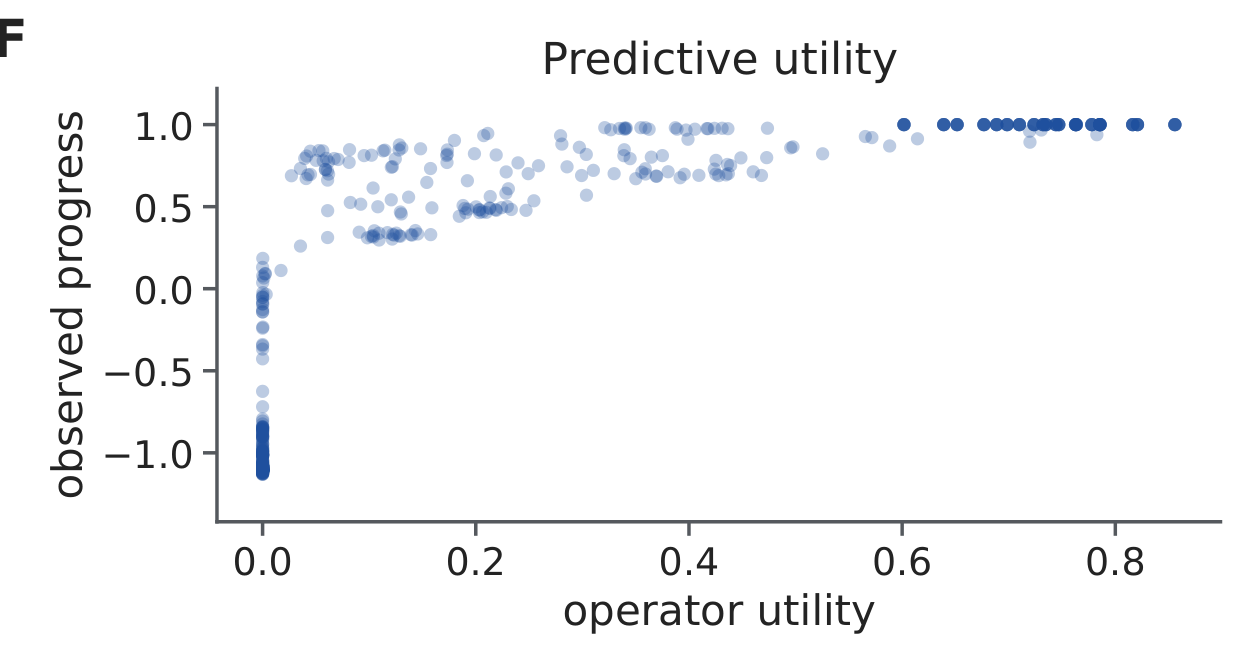
\includegraphics[width=6.55in]{operator_utility_validation.png}};
    \node[anchor=north east,text=ink,text width=6.25in,align=center,
      font=\sffamily\bfseries\fontsize{10.0}{12}\selectfont]
      at ($(current page.north east)+(-0.52in,-5.00in)$)
      {$\rho_s=0.937$ one-step \qquad $\rho_s=0.916$ final \qquad 540 controlled conditions};
    \node[anchor=north east,text=muted,text width=6.25in,align=center,
      font=\sffamily\itshape\fontsize{7.7}{9.0}\selectfont]
      at ($(current page.north east)+(-0.52in,-5.30in)$)
      {Exact for the isotropic quadratic; otherwise a smoothness bound that most directly predicts one-step progress.};

    \draw[ink!25,line width=0.8pt] ($(current page.north west)+(0.55in,-5.50in)$) --
      ($(current page.north east)+(-0.55in,-5.50in)$);
    \foreach \x/\col/\head/\txt in {
      1.75/green/alignment/{route span must capture useful credit},
      4.88/blue/bandwidth/{benefit can peak before full rank},
      8.10/purple/signal--noise/{rejected noise must offset discarded signal},
      11.18/orange/reliability/{gain helps when it follows signal-to-noise}}
    {
      \node[anchor=north,text=\col,font=\sffamily\bfseries\fontsize{9.4}{10.8}\selectfont]
        at ($(current page.north west)+(\x in,-5.76in)$) {\head};
      \node[anchor=north,text=ink,text width=2.70in,align=center,
        font=\sffamily\fontsize{7.9}{9.2}\selectfont]
        at ($(current page.north west)+(\x in,-6.10in)$) {\txt};
    }
  \end{tikzpicture}
  \takeaway{Operator utility balances aligned retained signal against routed update energy and admitted noise.}
\end{frame}

% 13 -------------------------------------------------------------------------
\begin{frame}[plain]
  \fullimage{assets/standard_task_setup.png}
  \begin{tikzpicture}[remember picture,overlay]
    \fill[white] (current page.north west) rectangle ($(current page.north east)+(0,-0.78in)$);
    \node[anchor=west,text=ink,font=\rmfamily\bfseries\fontsize{23}{26}\selectfont]
      at ($(current page.north west)+(0.44in,-0.36in)$)
      {Standard benchmarks vary feedback resolution while holding the forward model fixed};
    \draw[ink!78,line width=0.8pt]
      ($(current page.north west)+(0.44in,-0.76in)$) --
      ($(current page.north east)+(-0.44in,-0.76in)$);
    \fill[white] (current page.south west) rectangle ($(current page.south east)+(0,0.53in)$);
    \node[anchor=center,text=ink,text width=12.0in,align=center,
      font=\sffamily\bfseries\fontsize{9.7}{11.5}\selectfont]
      at ($(current page.south)+(0,0.27in)$)
      {The ladder asks first whether feedback must identify the neuron, then whether it must resolve locations within its arbor.};
  \end{tikzpicture}
\end{frame}

% 14 -------------------------------------------------------------------------
\begin{frame}[plain]
  \abstitle{Neuron identity closes almost the entire standard-task gap}
  \begin{tikzpicture}[remember picture,overlay]
    \node[anchor=north west,inner sep=0]
      at ($(current page.north west)+(0.40in,-1.08in)$)
      {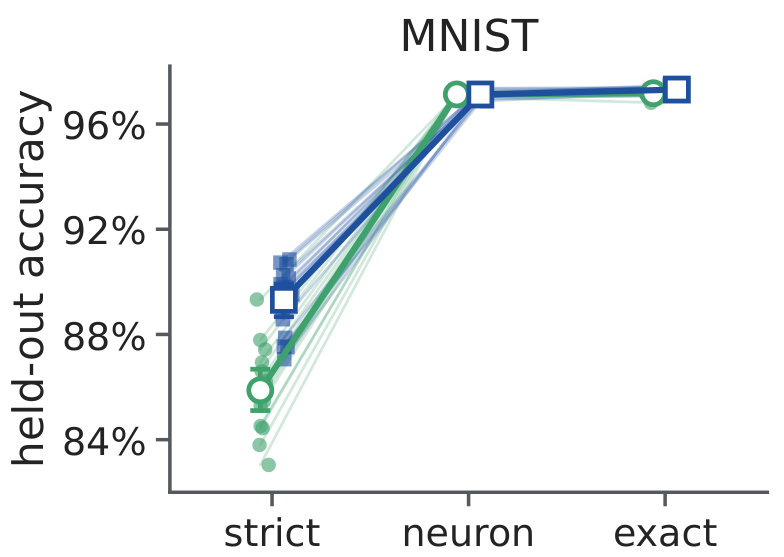
\includegraphics[height=4.20in]{mnist_strict_scalar.png}};
    \node[anchor=north west,inner sep=0]
      at ($(current page.north west)+(4.56in,-1.20in)$)
      {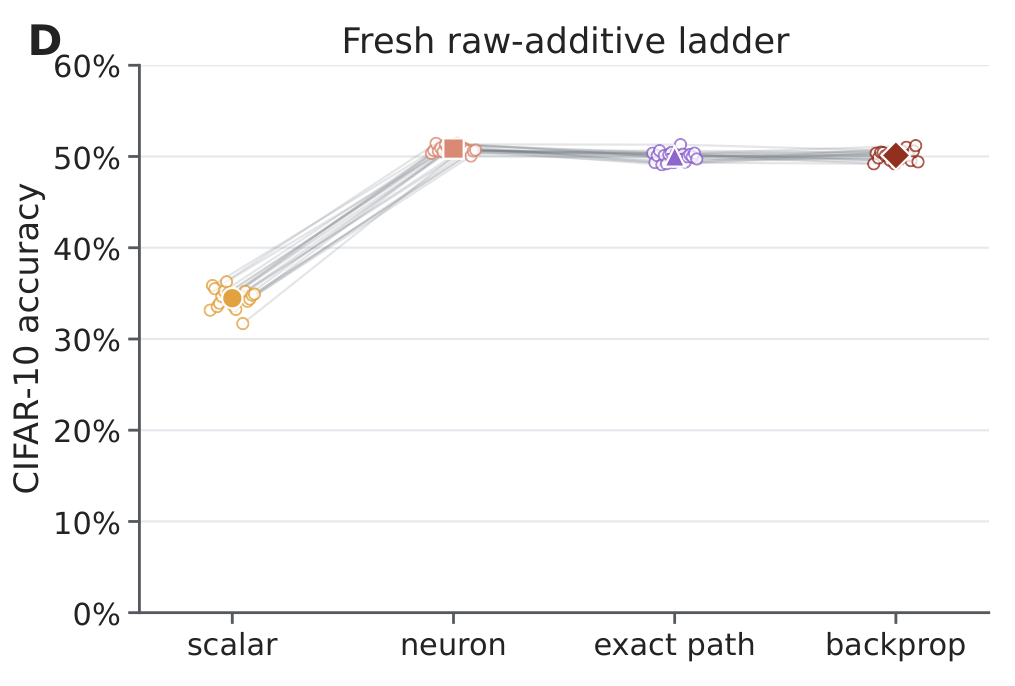
\includegraphics[width=5.00in]{cifar_confirmatory_ladder.png}};
    \node[anchor=north west,text=ink,text width=3.00in,align=left,
      font=\sffamily\fontsize{9.2}{11.0}\selectfont]
      at ($(current page.north west)+(9.92in,-1.25in)$)
      {\plainlabel{green}{MNIST}\\[-1pt]
       neuron-specific over strict scalar:\\[2pt]
       $+11.2$ pp shunting\\
       $+7.8$ pp raw additive\\[8pt]
       exact path over neuron-specific:\\[2pt]
       $<0.2$ pp};
    \node[anchor=north west,text=ink,text width=3.00in,align=left,
      font=\sffamily\fontsize{9.2}{11.0}\selectfont]
      at ($(current page.north west)+(9.92in,-3.72in)$)
      {\plainlabel{blue}{Flattened CIFAR-10}\\[-1pt]
       scalar $34.47\%$\\
       neuron-specific $50.87\%$\\
       exact path $50.01\%$\\
       matched BP $50.12\%$};

    \draw[ink!25,line width=0.8pt] ($(current page.north west)+(0.55in,-5.75in)$) --
      ($(current page.north east)+(-0.55in,-5.75in)$);
    \node[anchor=north west,text=muted,font=\sffamily\bfseries\fontsize{8.3}{9.6}\selectfont]
      at ($(current page.north west)+(0.70in,-6.01in)$) {DISTAL PATH-SPECIFIC ERROR ENERGY};
    \draw[green,line width=7pt] ($(current page.north west)+(4.04in,-6.15in)$) --
      ($(current page.north west)+(6.55in,-6.15in)$);
    \draw[blue,line width=7pt] ($(current page.north west)+(4.04in,-6.48in)$) --
      ($(current page.north west)+(5.55in,-6.48in)$);
    \node[anchor=east,text=green,font=\sffamily\bfseries\fontsize{9.3}{10.4}\selectfont]
      at ($(current page.north west)+(3.80in,-6.15in)$) {shunting};
    \node[anchor=east,text=blue,font=\sffamily\bfseries\fontsize{9.3}{10.4}\selectfont]
      at ($(current page.north west)+(3.80in,-6.48in)$) {raw additive};
    \node[anchor=west,text=green,font=\sffamily\bfseries\fontsize{9.3}{10.4}\selectfont]
      at ($(current page.north west)+(6.72in,-6.15in)$) {$\approx53\%$};
    \node[anchor=west,text=blue,font=\sffamily\bfseries\fontsize{9.3}{10.4}\selectfont]
      at ($(current page.north west)+(5.72in,-6.48in)$) {$\approx32\%$};
    \node[anchor=west,text=ink,text width=5.30in,align=left,
      font=\sffamily\fontsize{8.8}{10.5}\selectfont]
      at ($(current page.north west)+(7.15in,-6.08in)$)
      {Path-specific gradients exist, especially under shunting, but these benchmarks do not reward resolving them.};
  \end{tikzpicture}
\end{frame}

% 15 -------------------------------------------------------------------------
\begin{frame}[plain]
  \abstitle{Branch conflict creates a controlled need for an internal address}
  \begin{tikzpicture}[remember picture,overlay]
    \node[anchor=north west,inner sep=0]
      at ($(current page.north west)+(0.38in,-1.02in)$)
      {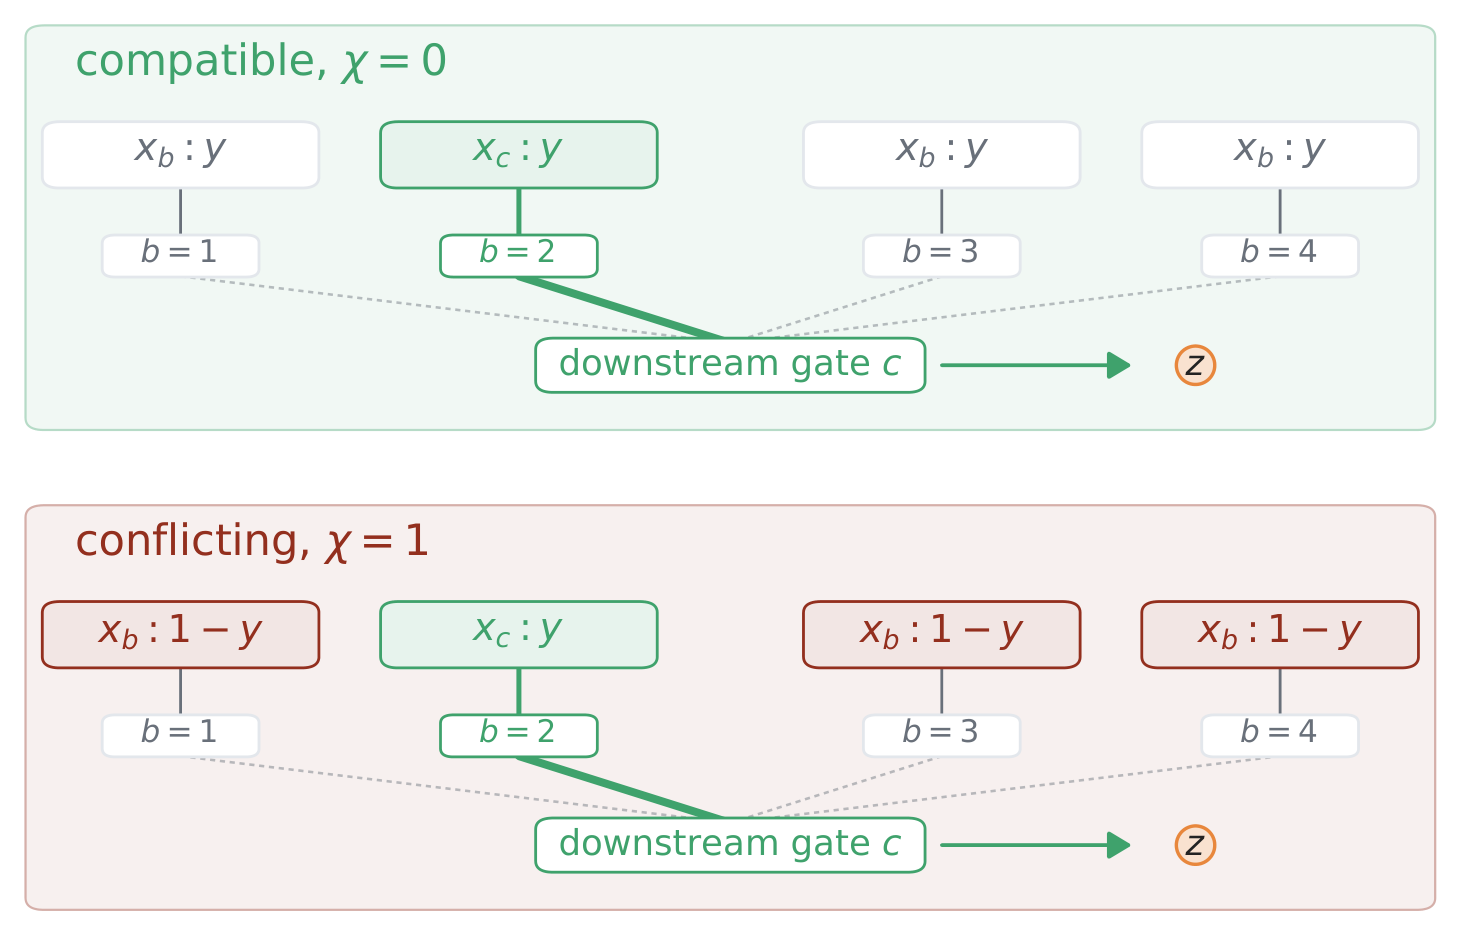
\includegraphics[width=7.55in]{path_necessity_task.png}};
    \node[anchor=north west,text=ink,align=left,text width=4.55in,
      font=\sffamily\fontsize{9.6}{11.7}\selectfont]
      at ($(current page.north west)+(8.18in,-1.12in)$)
      {All $B$ branches are active. Context $c$ selects the branch whose image class determines the label. Each nonselected branch carries the opposite-class view with probability $\chi$.};
    \node[anchor=north west,text=ink,text width=4.35in,align=center,
      font=\rmfamily\fontsize{15.2}{19}\selectfont]
      at ($(current page.north west)+(8.18in,-2.65in)$)
      {$\lambda_{\rm shared}=B-2\chi(B-1)$\\[5pt]
       $\displaystyle\chi_c=\frac{B}{2(B-1)}$};
    \draw[green,line width=2.0pt] ($(current page.north west)+(8.25in,-4.24in)$) --
      ($(current page.north west)+(8.95in,-4.24in)$);
    \node[anchor=west,text=ink,text width=3.65in,align=left,
      font=\sffamily\fontsize{9.2}{11.0}\selectfont]
      at ($(current page.north west)+(9.12in,-4.24in)$)
      {branch-specific credit preserves the selected local sign};
    \draw[purple,line width=2.0pt] ($(current page.north west)+(8.25in,-5.08in)$) --
      ($(current page.north west)+(8.95in,-5.08in)$);
    \node[anchor=west,text=ink,text width=3.65in,align=left,
      font=\sffamily\fontsize{9.2}{11.0}\selectfont]
      at ($(current page.north west)+(9.12in,-5.08in)$)
      {a neuron-shared signal cancels above the predicted $\chi_c$};
    \node[anchor=north west,text=muted,text width=4.55in,align=left,
      font=\sffamily\itshape\fontsize{8.5}{10.0}\selectfont]
      at ($(current page.north west)+(8.18in,-5.93in)$)
      {Mechanism-matched existence test; it is not intended to represent every natural task.};
  \end{tikzpicture}
  \takeaway{The task varies one interpretable quantity: how strongly sibling branches demand opposing updates.}
\end{frame}

% 16 -------------------------------------------------------------------------
\begin{frame}[plain]
  \abstitle{Shared credit fails at the predicted conflict boundary}
  \begin{tikzpicture}[remember picture,overlay]
    \node[anchor=north west,inner sep=0]
      at ($(current page.north west)+(0.48in,-1.02in)$)
      {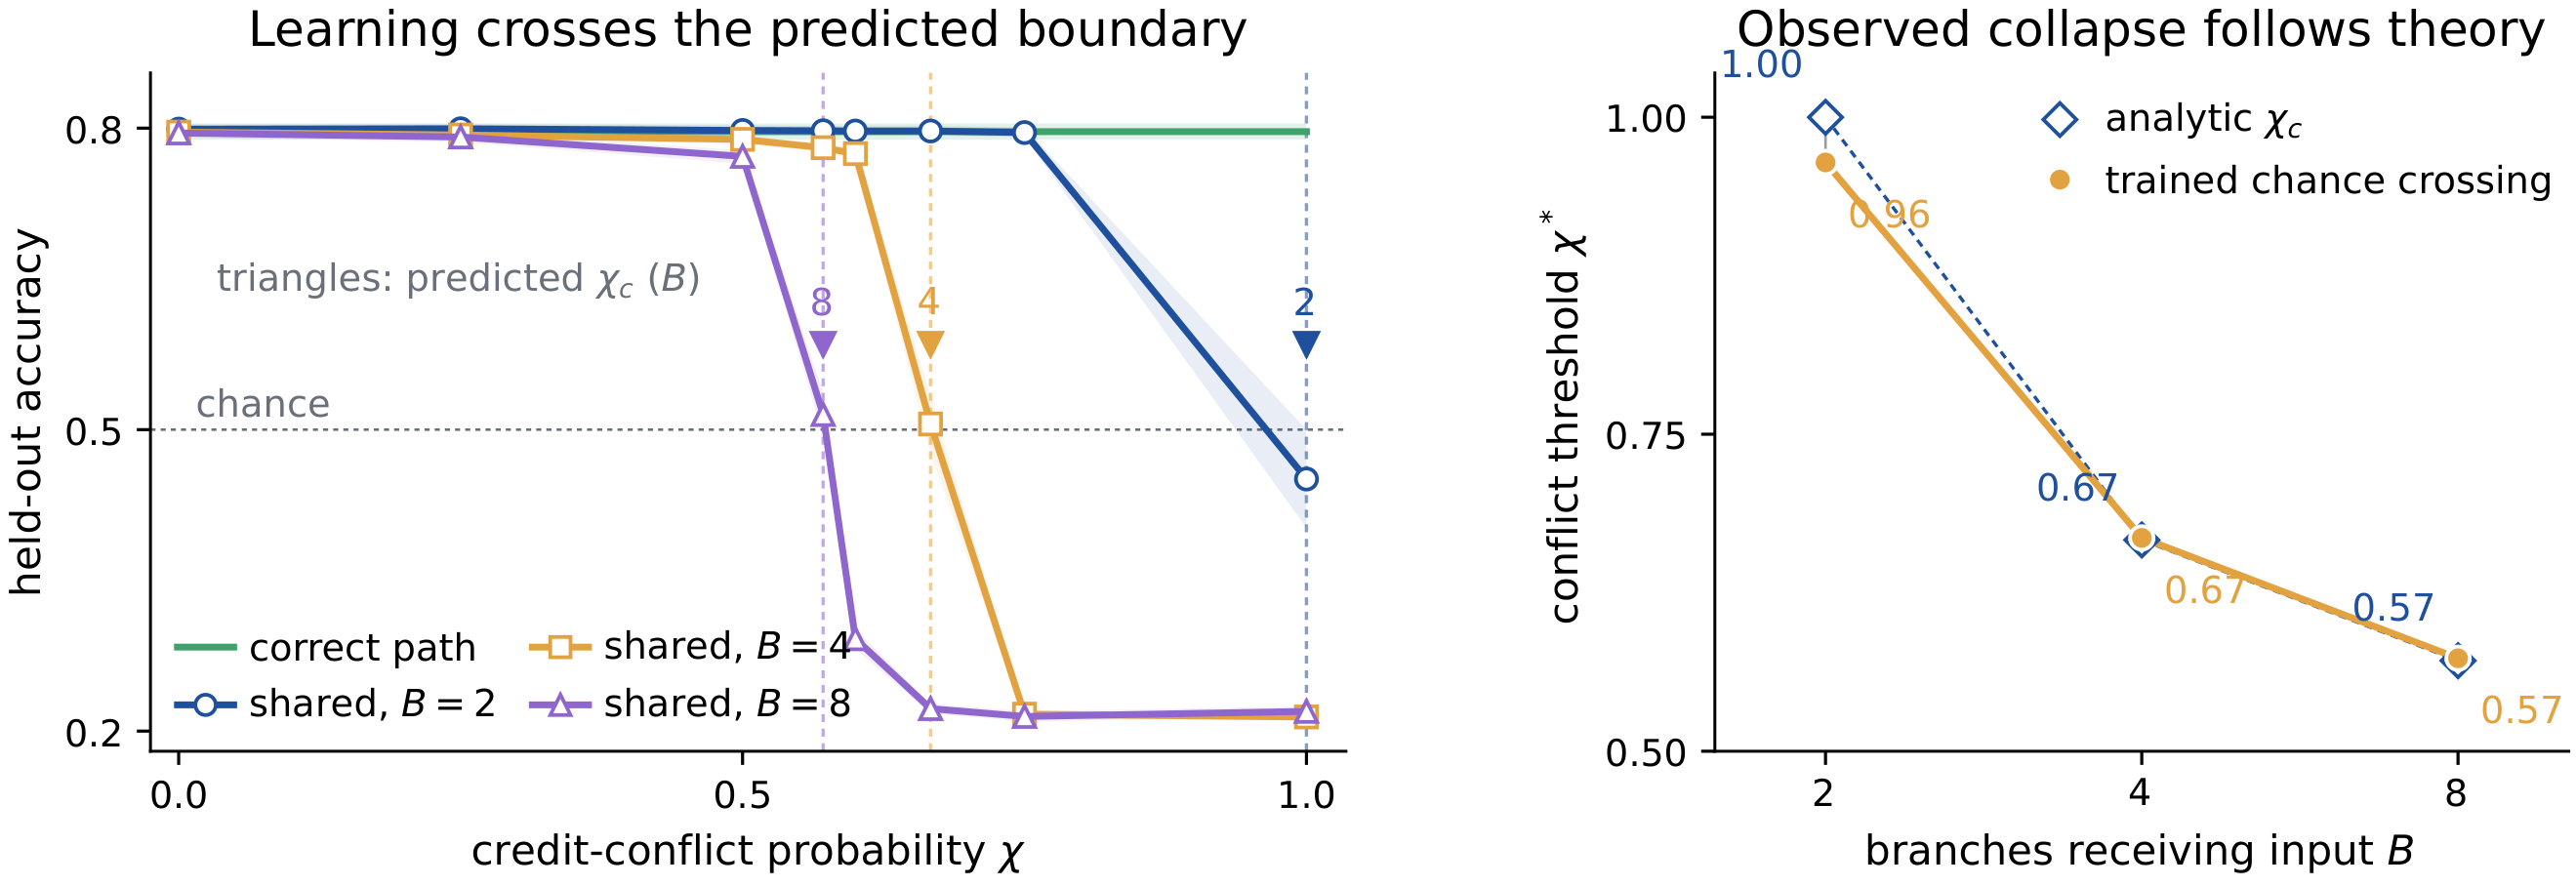
\includegraphics[width=12.35in]{path_necessity_results.png}};
    \node[anchor=north west,text=purple,text width=3.45in,align=center,
      font=\sffamily\bfseries\fontsize{10.0}{12}\selectfont]
      at ($(current page.north west)+(0.52in,-5.51in)$)
      {$\displaystyle \chi_c=\frac{B}{2(B-1)}$\\[-1pt]
       \normalfont\color{ink}\fontsize{8.3}{9.8}\selectfont analytic and trained crossings agree for $B\in\{2,4,8\}$};
    \node[anchor=north west,text=green,text width=3.15in,align=center,
      font=\sffamily\bfseries\fontsize{18}{20}\selectfont]
      at ($(current page.north west)+(4.50in,-5.51in)$)
      {35--58 pp\\[-1pt]
       \normalfont\color{ink}\fontsize{8.3}{9.8}\selectfont correct branch route over neuron-shared credit at full conflict};
    \node[anchor=north west,text=ink,text width=4.48in,align=left,
      font=\sffamily\fontsize{8.7}{10.4}\selectfont]
      at ($(current page.north west)+(8.07in,-5.51in)$)
      {A cyclic derangement preserves rank and sparsity but sends each value to the wrong branch. It fails across 20 seeds per $B$.};
  \end{tikzpicture}
  \takeaway{Feedback rank is not enough: the signal must reach the branch that owns the relevant eligibility.}
\end{frame}

% 17 -------------------------------------------------------------------------
\begin{frame}[plain]
  \abstitle{A hierarchical task tests subtree routes at limited feedback bandwidth}
  \begin{tikzpicture}[remember picture,overlay]
    \node[anchor=north west,inner sep=0]
      at ($(current page.north west)+(0.42in,-1.05in)$)
      {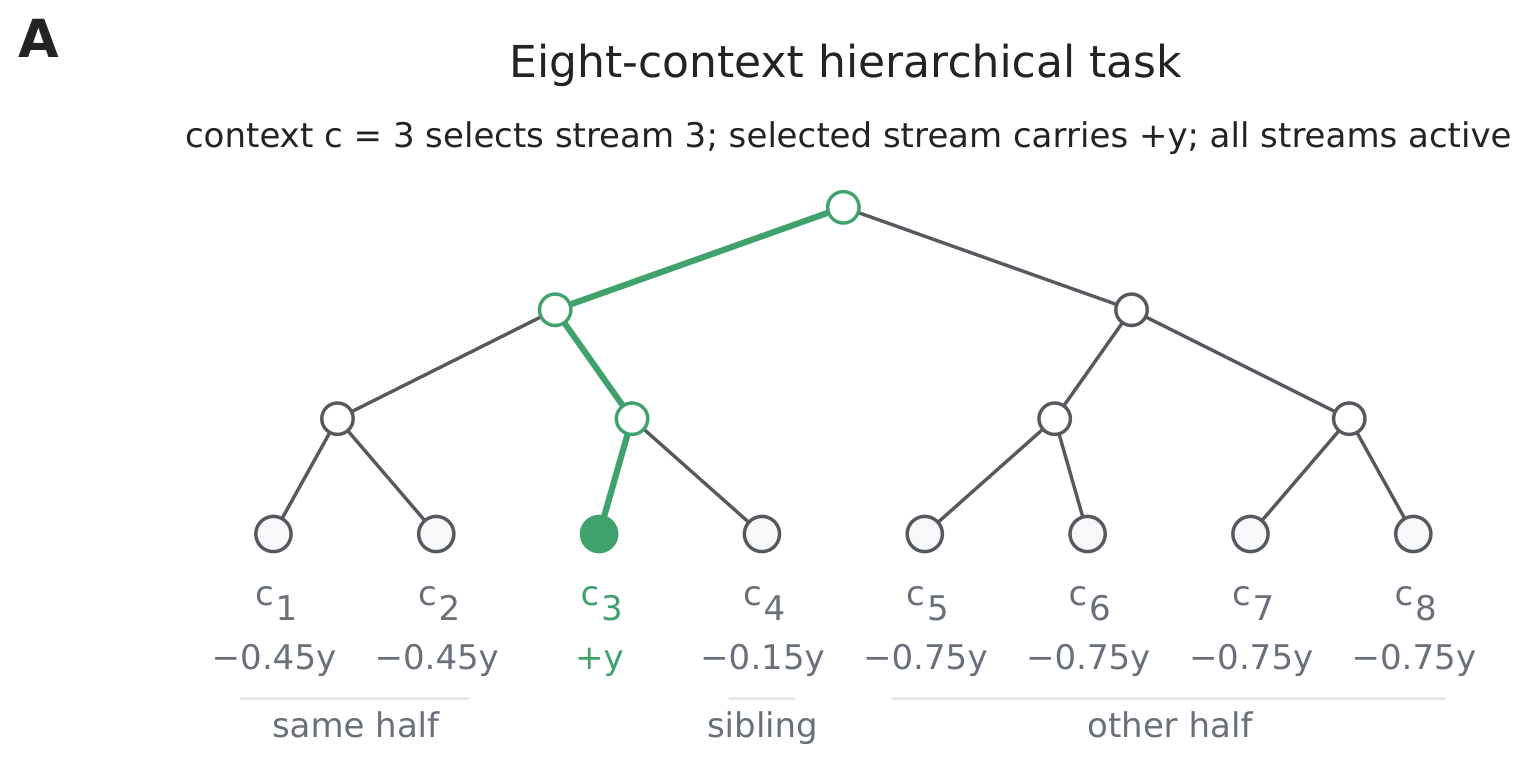
\includegraphics[width=6.20in,trim=22 0 0 0,clip]{hierarchy_task_current.png}};
    \node[anchor=north west,inner sep=0]
      at ($(current page.north west)+(7.06in,-1.12in)$)
      {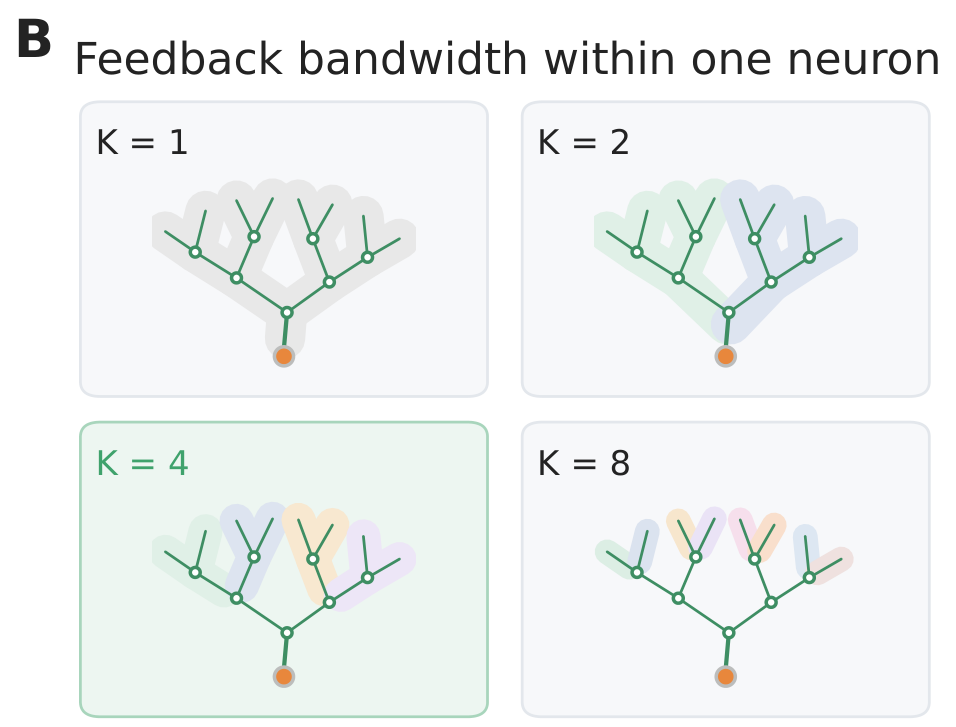
\includegraphics[width=3.30in,trim=20 0 0 0,clip]{hierarchy_bandwidth_current.png}};
    \node[anchor=north west,text=ink,text width=2.30in,align=left,
      font=\sffamily\fontsize{8.25}{9.8}\selectfont]
      at ($(current page.north west)+(10.58in,-1.18in)$)
      {Context selects one of eight active streams independently of the balanced label. The selected stream carries the label sign; opposite-sign distractor strength grows with tree distance.\\[5pt]
       $K=1,2,4,8$ is the number of independent route coefficients within one neuron.};
    \draw[ink!25,line width=0.8pt] ($(current page.north west)+(0.55in,-4.66in)$) --
      ($(current page.north east)+(-0.55in,-4.66in)$);
    \node[anchor=north west,text=green,text width=2.55in,align=left,
      font=\sffamily\bfseries\fontsize{9.5}{11}\selectfont]
      at ($(current page.north west)+(0.72in,-5.03in)$) {matched subtrees\\[-1pt]
      \normalfont\color{ink}correct supports on the known hierarchy};
    \node[anchor=north west,text=muted,text width=2.55in,align=left,
      font=\sffamily\bfseries\fontsize{9.5}{11}\selectfont]
      at ($(current page.north west)+(3.77in,-5.03in)$) {cyclic derangement\\[-1pt]
      \normalfont\color{ink}same routes, assigned to the wrong signals};
    \node[anchor=north west,text=purple,text width=2.55in,align=left,
      font=\sffamily\bfseries\fontsize{9.5}{11}\selectfont]
      at ($(current page.north west)+(6.82in,-5.03in)$) {dense low-rank basis\\[-1pt]
      \normalfont\color{ink}same feedback bandwidth, non-anatomical supports};
    \node[anchor=north west,text=blue,text width=2.55in,align=left,
      font=\sffamily\bfseries\fontsize{9.5}{11}\selectfont]
      at ($(current page.north west)+(9.87in,-5.03in)$) {rewired tree\\[-1pt]
      \normalfont\color{ink}degree and depth preserved, ancestry changed};
    \node[anchor=north,text=muted,text width=11.9in,align=center,
      font=\sffamily\fontsize{8.4}{9.8}\selectfont]
      at ($(current page.north)+(0,-6.27in)$)
      {$K$ is backward feedback bandwidth; it is not the number of serial dendritic stages $D_{\mathrm p}$ tested later.};
  \end{tikzpicture}
\end{frame}

% 18 -------------------------------------------------------------------------
\begin{frame}[plain]
  \abstitle{Correct assignment is essential; ancestry adds only a narrow $K=4$ gain}
  \begin{tikzpicture}[remember picture,overlay]
    \node[anchor=north west,inner sep=0]
      at ($(current page.north west)+(0.58in,-1.10in)$)
      {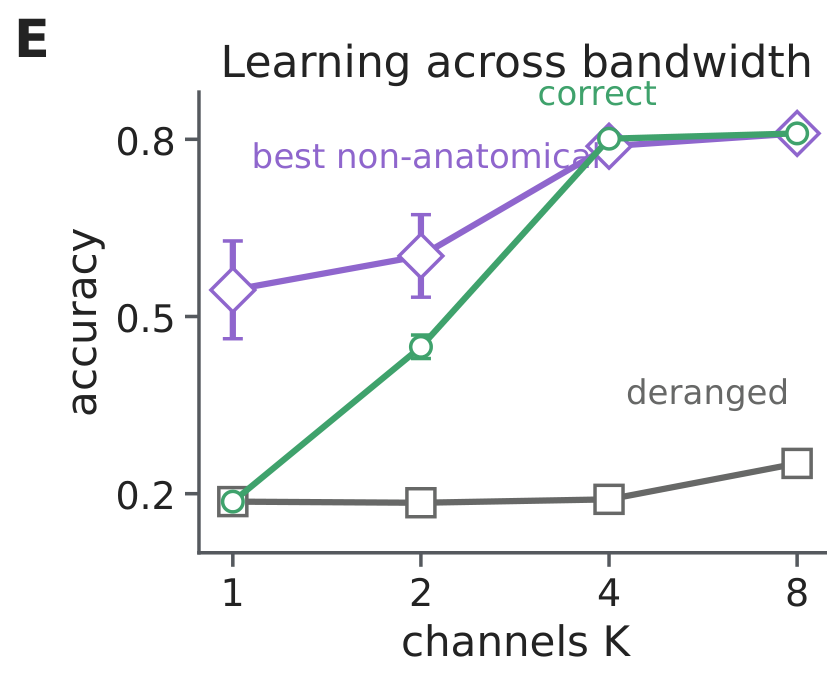
\includegraphics[width=7.15in,trim=22 0 0 0,clip]{hierarchy_learning_current.png}};
    \draw[ink!25,line width=0.8pt] ($(current page.north west)+(8.12in,-1.12in)$) --
      ($(current page.north west)+(8.12in,-5.70in)$);
    \node[anchor=north west,text=green,text width=4.25in,align=left,
      font=\sffamily\bfseries\fontsize{19}{21}\selectfont]
      at ($(current page.north west)+(8.55in,-1.36in)$) {+61.1 pp};
    \node[anchor=north west,text=ink,text width=4.15in,align=left,
      font=\sffamily\fontsize{9.8}{11.8}\selectfont]
      at ($(current page.north west)+(8.55in,-1.93in)$)
      {correct address versus cyclic derangement at $K=4$};
    \node[anchor=north west,text=purple,text width=4.25in,align=left,
      font=\sffamily\bfseries\fontsize{19}{21}\selectfont]
      at ($(current page.north west)+(8.55in,-3.05in)$) {+1.27 pp};
    \node[anchor=north west,text=ink,text width=4.15in,align=left,
      font=\sffamily\fontsize{9.8}{11.8}\selectfont]
      at ($(current page.north west)+(8.55in,-3.62in)$)
      {ancestry routes versus the strongest matched non-anatomical low-rank basis at $K=4$};
    \node[anchor=north west,text=muted,text width=4.10in,align=left,
      font=\sffamily\fontsize{8.7}{10.4}\selectfont]
      at ($(current page.north west)+(8.55in,-4.92in)$)
      {Most of the effect is correct delivery. The topology-specific increment disappears at low and full bandwidth.};
  \end{tikzpicture}
  \takeaway{Addresses can be essential, while the extra benefit of this particular nested topology is conditional and modest.}
\end{frame}

% 19 -------------------------------------------------------------------------
\begin{frame}[plain]
  \abstitle{Physical depth asks whether serial shunting matches a compositional task}
  \begin{tikzpicture}[remember picture,overlay]
    \node[anchor=north west,text=ink,font=\rmfamily\fontsize{15.8}{19}\selectfont]
      at ($(current page.north west)+(0.55in,-1.11in)$)
      {$\displaystyle x_j^E=s_y\prod_{\ell=1}^{H_{\mathrm p}}h_{\ell,a_\ell(j)}$};
    \node[anchor=north west,text=muted,text width=5.20in,align=left,
      font=\sffamily\fontsize{8.8}{10.4}\selectfont]
      at ($(current page.north west)+(0.58in,-1.98in)$)
      {$H_{\mathrm p}$ counts latent nuisance-gain levels in the task; $D_{\mathrm p}$ counts ordered nonlinear stages in the model.};
    \node[anchor=north west,inner sep=0]
      at ($(current page.north west)+(0.50in,-2.42in)$)
      {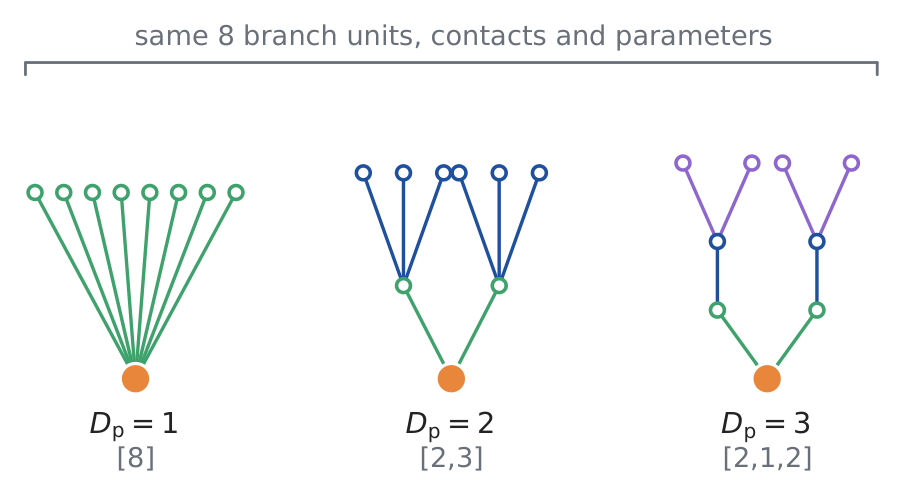
\includegraphics[width=5.56in]{physical_stage_schematic.png}};
    \node[anchor=north west,text=ink,text width=6.12in,align=left,
      font=\sffamily\fontsize{9.3}{11.2}\selectfont]
      at ($(current page.north west)+(6.53in,-1.10in)$)
      {\plainlabel{green}{Nested factors}\quad ordered cancellation of $h_1h_2h_3$\\[6pt]
       \plainlabel{blue}{Flat factors}\quad multiplicative factors distributed across non-nested groups\\[6pt]
       \plainlabel{purple}{Local ratios}\quad nuisance cancellation is available locally};
    \node[anchor=north west,text=muted,text width=6.02in,align=left,
      font=\sffamily\fontsize{7.9}{9.3}\selectfont]
      at ($(current page.north west)+(6.53in,-2.76in)$)
      {$\alpha=0$: independent sensors; $\alpha=1$: exact latent-gain sensors. Sensors are forward inhibitory inputs, not learning signals.};
    \draw[ink!25,line width=0.8pt] ($(current page.north west)+(6.53in,-3.40in)$) --
      ($(current page.north east)+(-0.56in,-3.40in)$);
    \node[anchor=north west,text=green,text width=1.80in,align=center,
      font=\sffamily\bfseries\fontsize{10}{11.6}\selectfont]
      at ($(current page.north west)+(6.60in,-3.75in)$) {serial tree\\
      \normalfont\color{ink}\fontsize{8.4}{9.8}\selectfont ordered stages};
    \node[anchor=north west,text=muted,text width=1.90in,align=center,
      font=\sffamily\bfseries\fontsize{10}{11.6}\selectfont]
      at ($(current page.north west)+(8.70in,-3.75in)$) {grouped point\\
      \normalfont\color{ink}\fontsize{8.4}{9.8}\selectfont same modules in parallel};
    \node[anchor=north west,text=blue,text width=1.90in,align=center,
      font=\sffamily\bfseries\fontsize{10}{11.6}\selectfont]
      at ($(current page.north west)+(10.95in,-3.75in)$) {point MLP\\
      \normalfont\color{ink}\fontsize{8.4}{9.8}\selectfont flexible ceiling};
    \begin{scope}[shift={($(current page.north west)+(7.50in,-5.38in)$)},x=1in,y=1in]
      \draw[green,line width=2.4pt] (0,0)--(0,0.42)--(0,0.84)--(0,1.26);
      \foreach \y in {0.42,0.84,1.26}{\draw[green,line width=2pt] (-0.20,\y)--(0.20,\y);}
      \fill[orange] (0,0) circle (0.085);
      \foreach \x in {1.55,1.87,2.19}{\node[draw=muted!60,fill=muted!10,minimum width=0.27in,minimum height=0.25in,inner sep=0] at (\x,1.0) {};\draw[muted!60] (\x,0.88)--(1.87,0.12);}
      \fill[orange] (1.87,0.12) circle (0.085);
      \foreach \x in {3.35,3.75,4.15}{\foreach \y in {0.2,0.7,1.2}{\fill[blue!45] (\x,\y) circle (0.045);}}
      \foreach \xa in {3.35,3.75}{\foreach \xb in {3.75,4.15}{\foreach \ya in {0.2,0.7,1.2}{\foreach \yb in {0.2,0.7,1.2}{\draw[blue!20] (\xa,\ya)--(\xb,\yb);}}}}
    \end{scope}
    \node[anchor=north west,text=muted,text width=6.02in,align=left,
      font=\sffamily\itshape\fontsize{8.4}{9.8}\selectfont]
      at ($(current page.north west)+(6.53in,-6.05in)$)
      {Mechanism-matched existence test at a calibrated divisive operating point; identical contacts and trainable resources for serial and grouped-point comparisons.};
  \end{tikzpicture}
\end{frame}

% 20 -------------------------------------------------------------------------
\begin{frame}[plain]
  \abstitle{Serial depth helps only when operation, order, and task are aligned}
  \begin{tikzpicture}[remember picture,overlay]
    \node[anchor=north west,inner sep=0]
      at ($(current page.north west)+(0.45in,-1.08in)$)
      {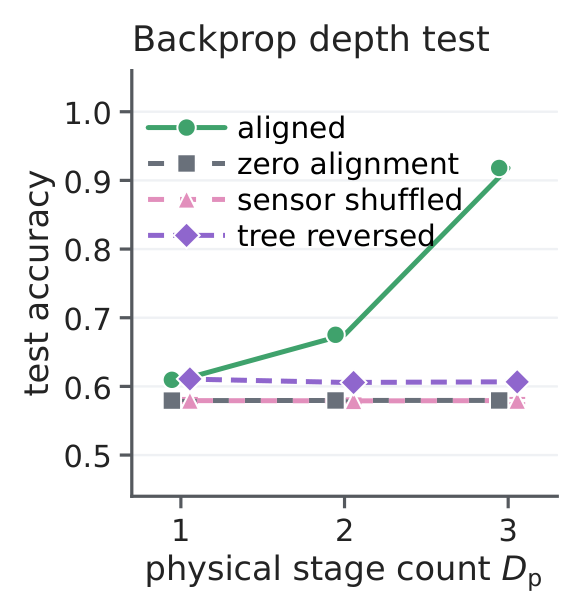
\includegraphics[height=4.55in]{physical_depth_headline.png}};
    \node[anchor=north west,inner sep=0]
      at ($(current page.north west)+(4.35in,-1.30in)$)
      {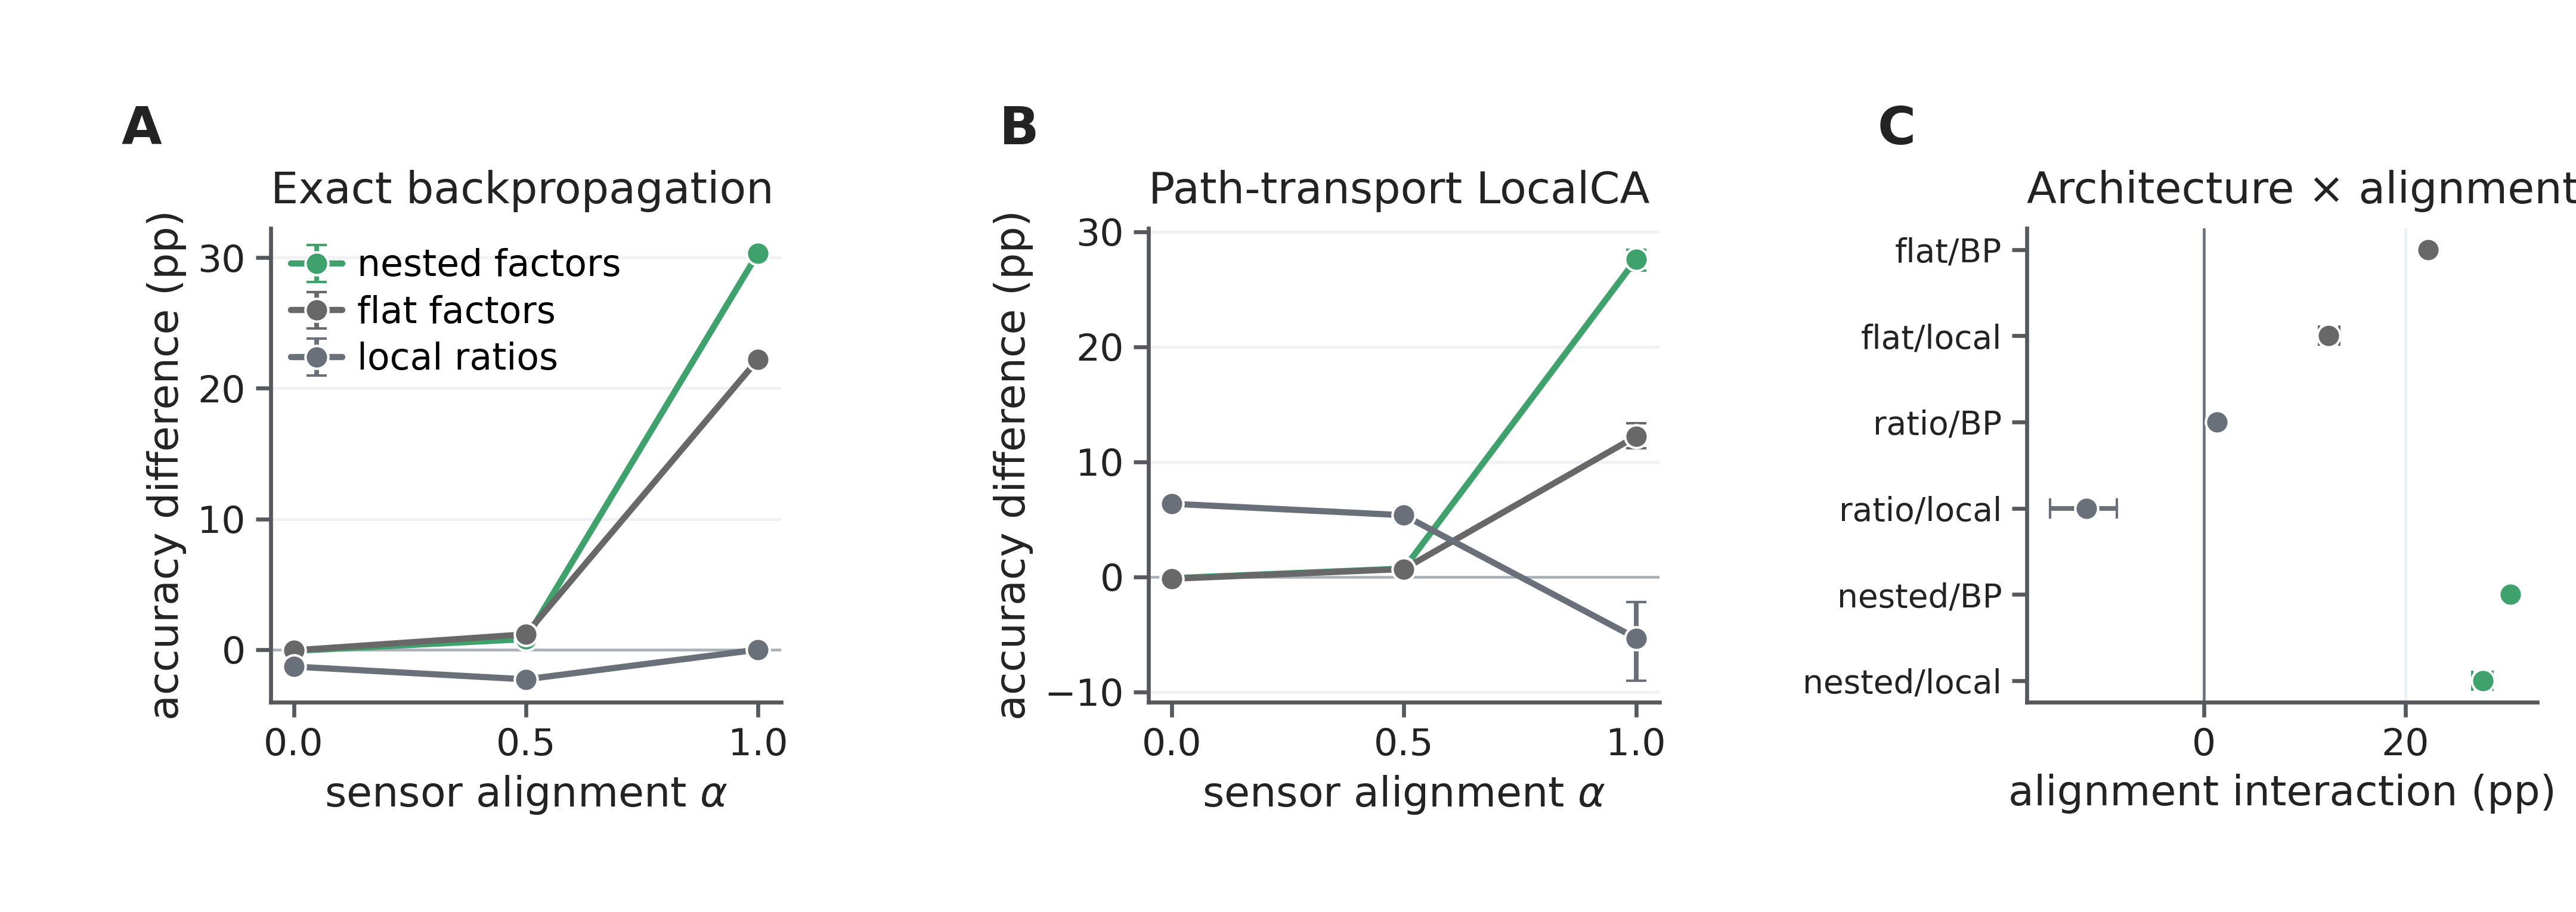
\includegraphics[width=8.50in]{../../journal/figures/generated/fig_task_family_alignment.png}};
    \draw[ink!25,line width=0.8pt] ($(current page.north west)+(0.55in,-5.58in)$) --
      ($(current page.north east)+(-0.55in,-5.58in)$);
    \node[anchor=north west,text=green,text width=2.30in,align=left,
      font=\sffamily\bfseries\fontsize{10.0}{11.6}\selectfont]
      at ($(current page.north west)+(0.70in,-5.90in)$) {+30.9 pp\\[-1pt]
      \normalfont\color{ink}\fontsize{8.2}{9.6}\selectfont aligned D3 versus D1 under BP};
    \node[anchor=north west,text=purple,text width=2.45in,align=left,
      font=\sffamily\bfseries\fontsize{10.0}{11.6}\selectfont]
      at ($(current page.north west)+(3.30in,-5.90in)$) {$\sim$11 pp\\[-1pt]
      \normalfont\color{ink}\fontsize{8.2}{9.6}\selectfont exact-path over shared-soma local credit at D3};
    \node[anchor=north west,text=blue,text width=2.45in,align=left,
      font=\sffamily\bfseries\fontsize{10.0}{11.6}\selectfont]
      at ($(current page.north west)+(6.05in,-5.90in)$) {controls\\[-1pt]
      \normalfont\color{ink}\fontsize{8.2}{9.6}\selectfont reversed sensors and raw-additive depth remove the benefit};
    \node[anchor=north west,text=orange,text width=3.65in,align=left,
      font=\sffamily\bfseries\fontsize{10.0}{11.6}\selectfont]
      at ($(current page.north west)+(8.80in,-5.90in)$) {boundary\\[-1pt]
      \normalfont\color{ink}\fontsize{8.2}{9.6}\selectfont useful depth saturates; a flexible point network remains the performance ceiling};
  \end{tikzpicture}
\end{frame}

% 21 -------------------------------------------------------------------------
\begin{frame}[plain]
  \abstitle{Reconstructed arbors provide sparse, predominantly coarse route dictionaries}
  \begin{tikzpicture}[remember picture,overlay]
    \node[anchor=north west,inner sep=0]
      at ($(current page.north west)+(0.55in,-1.15in)$)
      {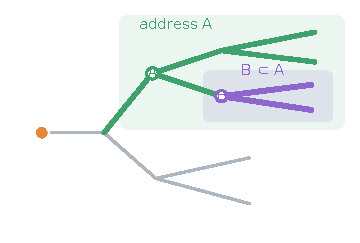
\includegraphics[width=3.45in]{../../journal/figures/components/main_ancestry_addresses.pdf}};
    \node[anchor=north west,inner sep=0]
      at ($(current page.north west)+(4.35in,-1.12in)$)
      {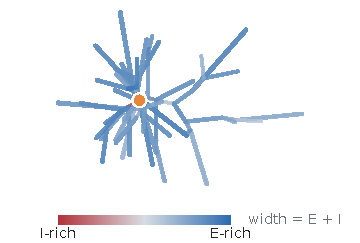
\includegraphics[width=3.15in]{../../journal/figures/components/main_mapped_reconstruction.pdf}};
    \node[anchor=north west,inner sep=0]
      at ($(current page.north west)+(7.72in,-1.20in)$)
      {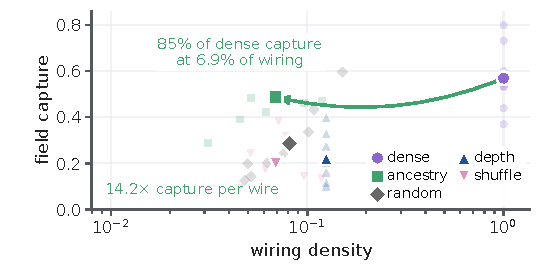
\includegraphics[width=5.05in]{../../journal/figures/components/main_wire_efficiency.pdf}};
    \draw[ink!25,line width=0.8pt] ($(current page.north west)+(0.55in,-4.70in)$) --
      ($(current page.north east)+(-0.55in,-4.70in)$);
    \node[anchor=north west,text=green,text width=2.25in,align=left,
      font=\sffamily\bfseries\fontsize{17}{19}\selectfont]
      at ($(current page.north west)+(0.72in,-5.03in)$) {$85\%$ capture};
    \node[anchor=north west,text=ink,text width=2.25in,align=left,
      font=\sffamily\fontsize{8.7}{10.4}\selectfont]
      at ($(current page.north west)+(0.72in,-5.61in)$) {with about $6.9\%$ of dense feedback connections};
    \node[anchor=north west,text=purple,text width=2.20in,align=left,
      font=\sffamily\bfseries\fontsize{17}{19}\selectfont]
      at ($(current page.north west)+(3.38in,-5.03in)$) {$14.2\times$};
    \node[anchor=north west,text=ink,text width=2.20in,align=left,
      font=\sffamily\fontsize{8.7}{10.4}\selectfont]
      at ($(current page.north west)+(3.38in,-5.61in)$) {model-matched capture-per-connection ceiling};
    \node[anchor=north west,text=blue,text width=2.30in,align=left,
      font=\sffamily\bfseries\fontsize{17}{19}\selectfont]
      at ($(current page.north west)+(6.02in,-5.03in)$) {$\sim2.7\times$};
    \node[anchor=north west,text=ink,text width=2.30in,align=left,
      font=\sffamily\fontsize{8.7}{10.4}\selectfont]
      at ($(current page.north west)+(6.02in,-5.61in)$) {density-matched anatomy-specific advantage};
    \node[anchor=north west,text=muted,text width=4.05in,align=left,
      font=\sffamily\fontsize{8.6}{10.2}\selectfont]
      at ($(current page.north west)+(8.78in,-5.03in)$)
      {Primary extension: a disjoint 47-cell cohort reproduces the route ordering. All ten qualifying cells from a second mouse show the model-matched subtree advantage. These are modeled fields on measured anatomy, not observed task gradients.};
  \end{tikzpicture}
\end{frame}

% 22 -------------------------------------------------------------------------
\begin{frame}[plain]
  \abstitle{Focal shunting regulates route gain only in a permissive conductance regime}
  \begin{tikzpicture}[remember picture,overlay]
    \begin{scope}[shift={($(current page.north west)+(0.42in,-1.04in)$)},x=1in,y=1in]
      \fill[paleblue] (0,0) rectangle (2.70,-2.48);
      \draw[blue!38,line width=0.7pt] (0,0) rectangle (2.70,-2.48);
      \node[anchor=north,font=\sffamily\bfseries\fontsize{9.0}{10.4}\selectfont,text=blue]
        at (1.35,-0.14) {current-matched injection};
      \coordinate (ls) at (1.35,-2.13); \coordinate (lk) at (1.35,-1.47);
      \draw[green!72!black,line width=2.0pt] (ls)--(1.35,-1.73)--(lk)--(0.72,-0.95);
      \draw[green!72!black,line width=2.0pt] (lk)--(2.00,-0.98);
      \draw[green!72!black,line width=1.45pt] (0.72,-0.95)--(0.42,-0.64) (0.72,-0.95)--(0.92,-0.56);
      \draw[green!72!black,line width=1.45pt] (2.00,-0.98)--(1.76,-0.62) (2.00,-0.98)--(2.32,-0.63);
      \fill[orange] (ls) circle (0.095); \draw[red,line width=1.5pt,fill=white] (lk) circle (0.055);
      \draw[->,blue,line width=2.0pt] (0.18,-1.47)--(1.24,-1.47);
      \node[anchor=south,text=blue,font=\sffamily\bfseries\fontsize{8.7}{9.6}\selectfont]
        at (0.62,-1.43) {$I_k^{\rm match}$};
      \draw[->,muted,line width=1.8pt] (2.83,-1.25)--(3.12,-1.25);
      \fill[paleteal] (3.24,0) rectangle (5.94,-2.48);
      \draw[green!42,line width=0.7pt] (3.24,0) rectangle (5.94,-2.48);
      \node[anchor=north,font=\sffamily\bfseries\fontsize{9.0}{10.4}\selectfont,text=green]
        at (4.59,-0.14) {focal inhibitory conductance};
      \coordinate (rs) at (4.59,-2.13); \coordinate (rk) at (4.59,-1.47);
      \draw[muted!45,line width=1.3pt] (rs)--(4.59,-1.73)--(rk)--(3.96,-0.95);
      \draw[green,line width=3.0pt] (rk)--(5.24,-0.98);
      \draw[muted!45,line width=1.1pt] (3.96,-0.95)--(3.66,-0.64) (3.96,-0.95)--(4.16,-0.56);
      \draw[green,line width=2.2pt] (5.24,-0.98)--(5.00,-0.62) (5.24,-0.98)--(5.56,-0.63);
      \fill[orange] (rs) circle (0.095); \draw[red,line width=2.0pt,fill=white] (rk) circle (0.072);
      \node[anchor=west,text=red,font=\sffamily\bfseries\fontsize{8.7}{9.6}\selectfont]
        at (4.72,-1.43) {$G_k^I$};
    \end{scope}
    \node[anchor=north east,inner sep=0]
      at ($(current page.north east)+(-0.34in,-1.03in)$)
      {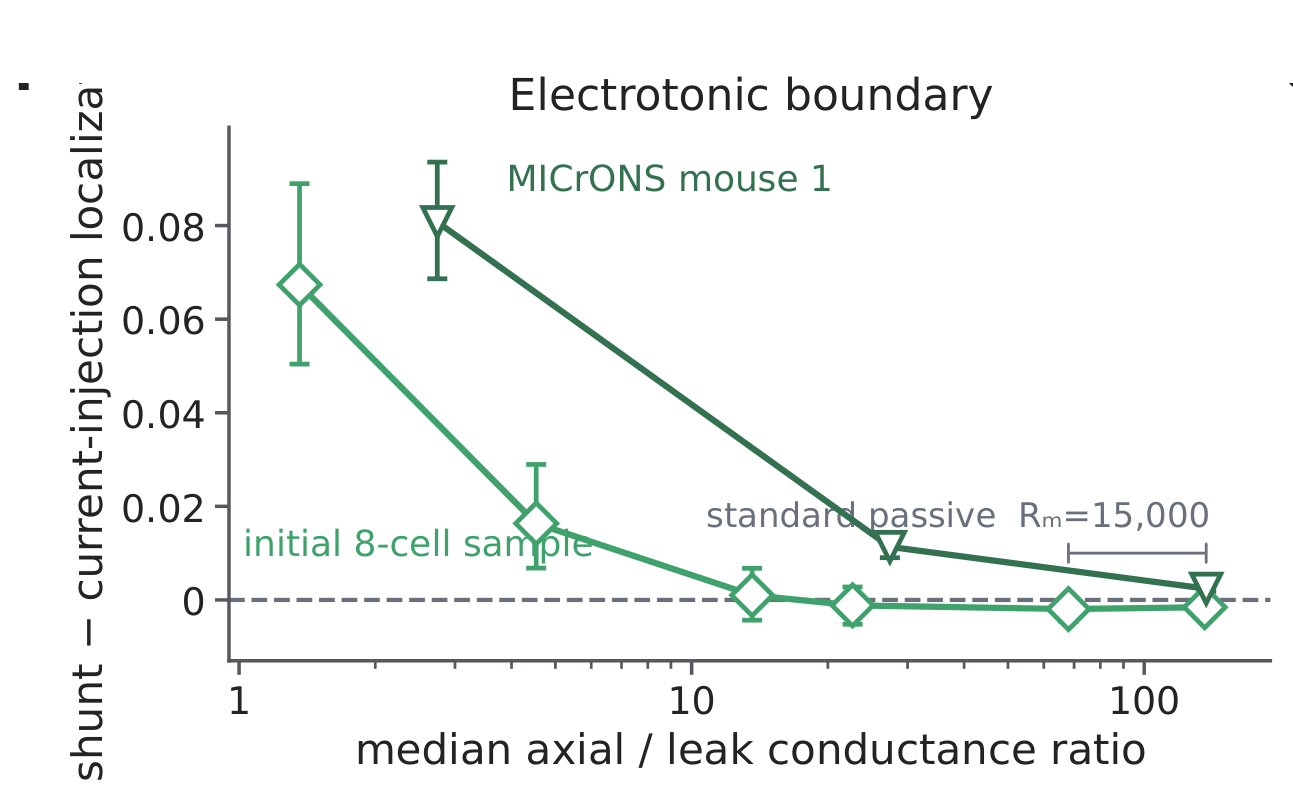
\includegraphics[width=6.08in]{focal_boundary_current.png}};
    \node[anchor=north west,text=ink,align=center,text width=5.54in]
      at ($(current page.north west)+(0.48in,-3.86in)$)
      {\fontsize{14}{17}\selectfont
      $\displaystyle
      \frac{\partial\log \alpha_n^{\rm cond}}{\partial G_k^I}
      =-R_k^{\rm tot}\,\mathbf 1\!\left[k\in\mathcal A(n)\right]$\\[-1pt]
      {\sffamily\fontsize{8.8}{10.4}\selectfont first-order change is restricted to descendants whose route passes through site $k$}};
    \node[anchor=north west,text=ink,align=left,text width=5.54in,
      font=\sffamily\fontsize{8.8}{10.4}\selectfont]
      at ($(current page.north west)+(0.48in,-5.20in)$)
      {Somatic voltage is restored after both interventions. Only the shunt changes $G$, and therefore $q=G^{-\top}\nabla_V\mathcal L$.};
    \node[anchor=north east,text=ink,align=left,text width=5.53in,
      font=\sffamily\fontsize{9.2}{11.1}\selectfont]
      at ($(current page.north east)+(-0.48in,-5.00in)$)
      {\textbf{Standard passive calibration} ($R_m=15{,}000\,\Omega\,\mathrm{cm}^2$): null.\\[3pt]
       \textbf{Lower resistance / background conductance}: descendant localization emerges.};
  \end{tikzpicture}
  \takeaway{Shunting can regulate an addressed route, but spatial selectivity is state dependent rather than automatic.}
\end{frame}

% 23 -------------------------------------------------------------------------
\begin{frame}[plain]
  \abstitle{Measured visual responses do not preferentially align with ancestry routes}
  \begin{tikzpicture}[remember picture,overlay]
    \node[anchor=north west,text=ink,text width=3.10in,align=left,
      font=\sffamily\fontsize{9.5}{11.4}\selectfont]
      at ($(current page.north west)+(0.58in,-1.23in)$)
      {Measured presynaptic visual responses are mapped to dendritic compartments on each reconstructed target cell. Each route dictionary predicts the target cell's held-out visual response.};
    \begin{scope}[shift={($(current page.north west)+(1.00in,-3.06in)$)},x=1in,y=1in]
      \coordinate (s) at (0.95,-1.55);
      \draw[green!75!black,line width=2.2pt] (s)--(0.95,-0.92)--(0.30,-0.22);
      \draw[green!75!black,line width=2.2pt] (0.95,-0.92)--(1.63,-0.28);
      \draw[green!75!black,line width=1.5pt] (0.30,-0.22)--(0.00,0.22) (0.30,-0.22)--(0.53,0.23);
      \draw[green!75!black,line width=1.5pt] (1.63,-0.28)--(1.35,0.18) (1.63,-0.28)--(1.98,0.18);
      \fill[orange] (s) circle (0.10);
      \foreach \x/\col in {0.00/blue,0.53/purple,1.35/blue,1.98/purple}{\fill[\col] (\x,0.22) circle (0.055);}
      \draw[->,ink!45,line width=1.5pt] (2.25,-0.65)--(3.15,-0.65);
      \node[anchor=south,text=ink,text width=1.50in,align=center,
        font=\sffamily\fontsize{8.4}{9.7}\selectfont]
        at (2.70,-0.53) {predict held-out response};
    \end{scope}
    \draw[ink!24,line width=0.8pt] ($(current page.north west)+(4.08in,-1.05in)$) --
      ($(current page.north west)+(4.08in,-5.82in)$);
    \node[anchor=north west,inner sep=0]
      at ($(current page.north west)+(4.42in,-1.28in)$)
      {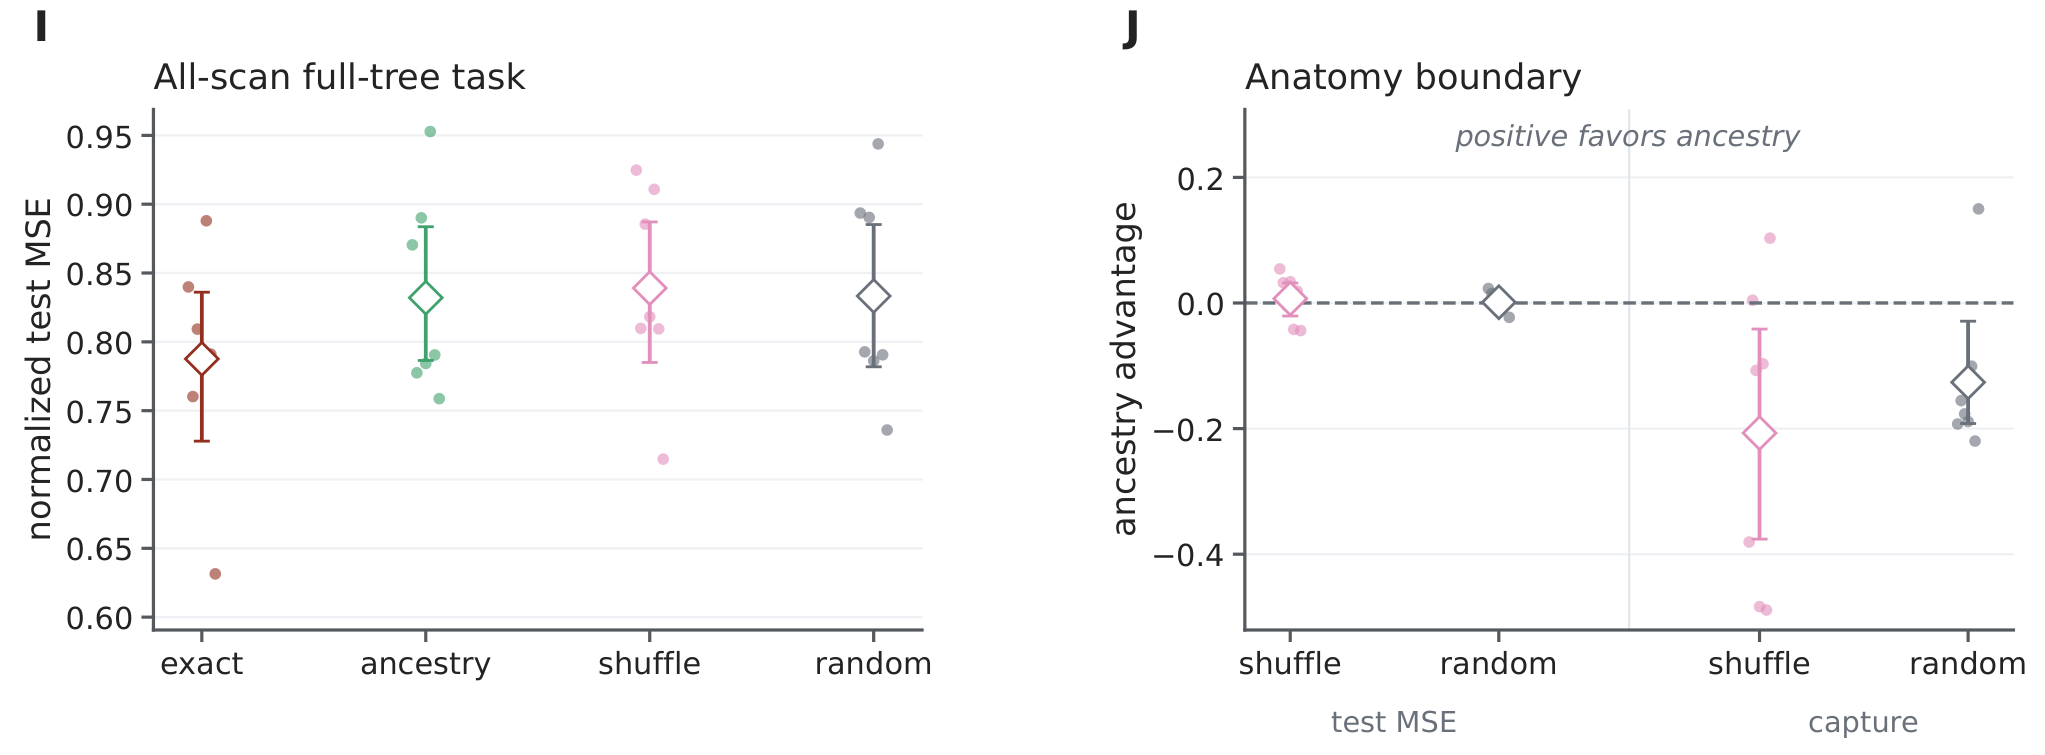
\includegraphics[width=8.28in]{fulltree_no_signed.png}};
    \node[anchor=north west,text=ink,text width=3.10in,align=left,
      font=\sffamily\bfseries\fontsize{10.0}{11.8}\selectfont]
      at ($(current page.north west)+(0.58in,-5.35in)$)
      {Seven target cells from one MICrONS mouse};
    \node[anchor=north,text=muted,text width=11.8in,align=center,
      font=\sffamily\fontsize{9.2}{10.9}\selectfont]
      at ($(current page.north)+(0,-6.06in)$)
      {Topology-minus-matched-control effects cross zero. Morphology supplies candidate routes, but this measured task does not establish their endogenous use.};
  \end{tikzpicture}
\end{frame}

% 24 -------------------------------------------------------------------------
\begin{frame}[plain]
  \abstitle{The same anatomy becomes useful when credit is rotated into its route span}
  \begin{tikzpicture}[remember picture,overlay]
    \node[anchor=north west,text=ink,font=\rmfamily\fontsize{15}{18}\selectfont]
      at ($(current page.north west)+(0.55in,-1.10in)$)
      {$\phi(a)=\sqrt a\,u_{\parallel}+\sqrt{1-a}\,u_{\perp},\qquad C_A[\phi(a)]=a$};
    \node[anchor=north west,inner sep=0]
      at ($(current page.north west)+(0.50in,-1.85in)$)
      {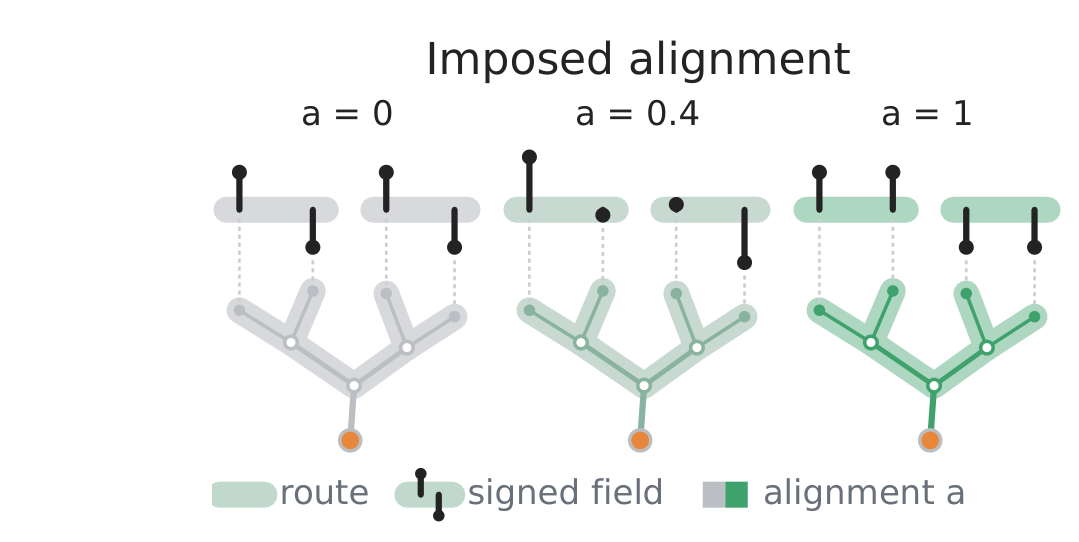
\includegraphics[width=6.15in]{alignment_rotation.png}};
    \draw[ink!24,line width=0.8pt] ($(current page.north west)+(6.72in,-1.06in)$) --
      ($(current page.north west)+(6.72in,-5.76in)$);
    \node[anchor=north west,inner sep=0]
      at ($(current page.north west)+(7.05in,-1.26in)$)
      {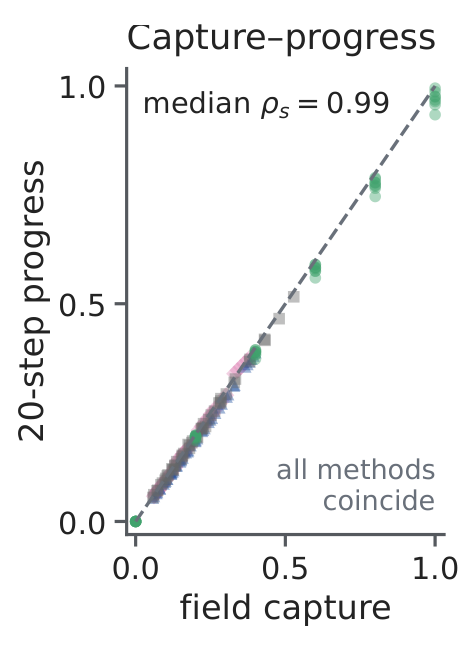
\includegraphics[height=4.45in]{alignment_rescue_n.png}};
    \node[anchor=north west,text=green,text width=1.52in,align=left,
      font=\sffamily\bfseries\fontsize{16}{18}\selectfont]
      at ($(current page.north west)+(11.18in,-1.58in)$) {8/8\\[-1pt]
      \normalfont\color{ink}\fontsize{8.5}{10}\selectfont lose at $a=0$, win at $a=1$};
    \node[anchor=north west,text=purple,text width=1.52in,align=left,
      font=\sffamily\bfseries\fontsize{15}{17}\selectfont]
      at ($(current page.north west)+(11.18in,-3.10in)$) {$\rho_s=0.99$\\[-1pt]
      \normalfont\color{ink}\fontsize{8.5}{10}\selectfont capture--progress};
    \node[anchor=north west,text=ink,text width=5.90in,align=left,
      font=\sffamily\fontsize{9.3}{11.1}\selectfont]
      at ($(current page.north west)+(0.55in,-5.43in)$)
      {Anatomy, route energy, and curvature remain fixed; only the task-credit field rotates from orthogonal to aligned.};
    \node[anchor=north west,text=muted,text width=5.55in,align=left,
      font=\sffamily\itshape\fontsize{8.5}{10}\selectfont]
      at ($(current page.north west)+(7.05in,-5.73in)$)
      {Alignment is imposed, not learned or observed endogenously.};
  \end{tikzpicture}
  \takeaway{This is a sufficiency test: fixed routes help when the required credit field lies in their span.}
\end{frame}

% 25 -------------------------------------------------------------------------
\begin{frame}[plain]
  \abstitle{Dendritic benefit requires a match among coordinate, address, gain, and task}
  \begin{tikzpicture}[remember picture,overlay]
    \node[anchor=north west,inner sep=0]
      at ($(current page.north west)+(0.44in,-1.02in)$)
      {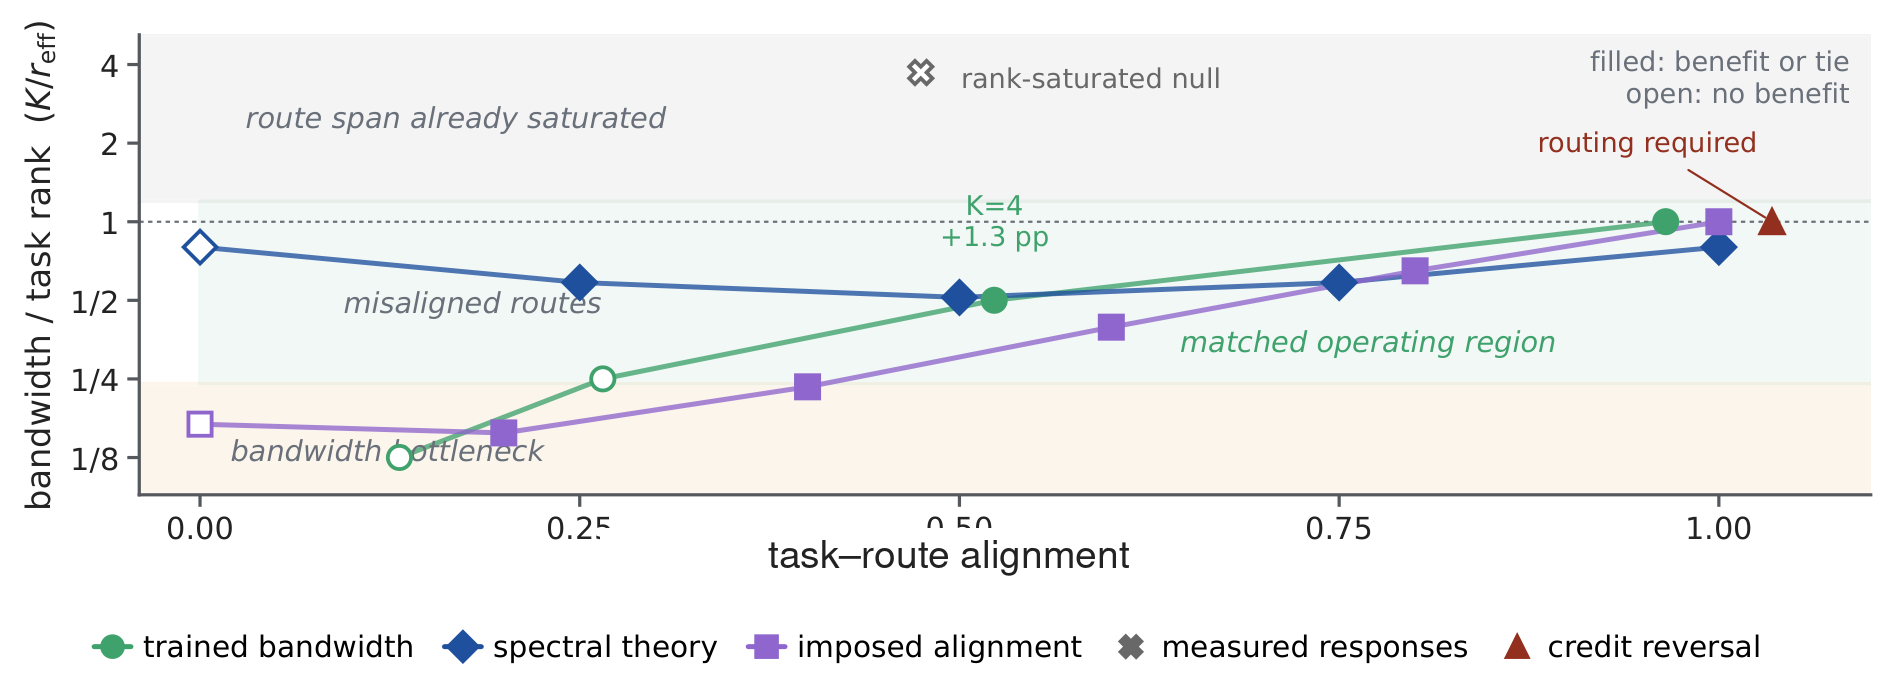
\includegraphics[width=12.44in]{phase_plane.png}};
    \node[anchor=north west,text=muted,font=\sffamily\itshape\fontsize{8.2}{9.4}\selectfont]
      at ($(current page.north west)+(0.58in,-5.55in)$)
      {theoretical regime map; boundaries are not fitted};
    \fill[white] ($(current page.north west)+(9.95in,-4.94in)$) rectangle
      ($(current page.north west)+(12.88in,-5.49in)$);
    \node[anchor=center,text=red,font=\sffamily\fontsize{11.0}{12}\selectfont]
      at ($(current page.north west)+(10.10in,-5.20in)$) {$\blacktriangle$};
    \node[anchor=west,text=red,font=\sffamily\bfseries\fontsize{8.8}{10.2}\selectfont]
      at ($(current page.north west)+(10.27in,-5.20in)$)
      {two-stream reversal ($K=2$)};
    \draw[ink!25,line width=0.8pt] ($(current page.north west)+(0.55in,-5.78in)$) --
      ($(current page.north east)+(-0.55in,-5.78in)$);
    \node[anchor=north west,text=blue,text width=2.78in,align=left,
      font=\sffamily\bfseries\fontsize{8.9}{10.4}\selectfont]
      at ($(current page.north west)+(0.60in,-6.00in)$) {Coordinate\\[-1pt]
      \normalfont\color{ink}neuron identity closes most of the standard-task gap};
    \node[anchor=north west,text=purple,text width=2.78in,align=left,
      font=\sffamily\bfseries\fontsize{8.9}{10.4}\selectfont]
      at ($(current page.north west)+(3.72in,-6.00in)$) {Address\\[-1pt]
      \normalfont\color{ink}routes help when local credits conflict};
    \node[anchor=north west,text=orange,text width=2.78in,align=left,
      font=\sffamily\bfseries\fontsize{8.9}{10.4}\selectfont]
      at ($(current page.north west)+(6.85in,-6.00in)$) {Gain and computation\\[-1pt]
      \normalfont\color{ink}shunting and serial depth help only in matched regimes};
    \node[anchor=north west,text=green,text width=2.78in,align=left,
      font=\sffamily\bfseries\fontsize{8.9}{10.4}\selectfont]
      at ($(current page.north west)+(9.98in,-6.00in)$) {Biological boundary\\[-1pt]
      \normalfont\color{ink}sparse capacity exists; endogenous alignment remains open};
  \end{tikzpicture}
  \takeaway{Dendrites are a conditional substrate for routing and transforming local credit---not a general replacement for backpropagation.}
\end{frame}

\end{document}
